	
\documentclass[conference]{IEEEtran}

% Some very useful LaTeX packages include:
% (uncomment the ones you want to load)

% *** MISC UTILITY PACKAGES ***
%
%\usepackage{ifpdf}
% Heiko Oberdiek's ifpdf.sty is very useful if you need conditional
% compilation based on whether the output is pdf or dvi.
% usage:
% \ifpdf
%   % pdf code
% \else
%   % dvi code
% \fi
% The latest version of ifpdf.sty can be obtained from:
% http://www.ctan.org/pkg/ifpdf
% Also, note that IEEEtran.cls V1.7 and later provides a builtin
% \ifCLASSINFOpdf conditional that works the same way.
% When switching from latex to pdflatex and vice-versa, the compiler may
% have to be run twice to clear warning/error messages.

\usepackage[english]{babel}
\usepackage[usenames]{color}
\usepackage{colortbl}
\usepackage{comment}
\usepackage{epsfig}
\usepackage{array, colortbl}
\usepackage{listings}
\usepackage{epstopdf}
\usepackage{multirow}
\usepackage{rotating}
\usepackage{subfigure}
\usepackage{subfig}
\usepackage{float}
%\usepackage[obeyspaces,hyphens,spaces]{url}
\usepackage{balance}
\usepackage{fancybox}
\usepackage{scalefnt}
\usepackage[normalem]{ulem}
\usepackage[export]{adjustbox}% http://ctan.org/pkg/adjustbox
\usepackage[table,xcdraw]{xcolor}
\usepackage{babel,blindtext}
\usepackage{graphicx}
\graphicspath{{./pdfs}{../pdfs/}}
\usepackage{cite}
\usepackage{float}

\usepackage{amsmath}

\usepackage{listings}
\usepackage{color}
\usepackage{inconsolata}
\definecolor{dkgreen}{rgb}{0,0.6,0}
\definecolor{gray}{rgb}{0.5,0.5,0.5}
\definecolor{mauve}{rgb}{0.58,0,0.82}
\definecolor{lightgray}{rgb}{.9,.9,.9}
\definecolor{darkgray}{rgb}{.4,.4,.4}
\definecolor{purple}{rgb}{0.65, 0.12, 0.82}

\lstdefinelanguage{JavaScript}{
  keywords={typeof, new, true, false, catch, function, return, null, catch, switch, var, if, in, while, do, else, case, break},
  keywordstyle=\color{blue}\bfseries,
  ndkeywords={class, export, boolean, throw, implements, import, this},
  ndkeywordstyle=\color{darkgray}\bfseries,
  identifierstyle=\color{black},
  sensitive=false,
  numbersep=1pt,
  xleftmargin=\parindent,
  comment=[l]{//},
  morecomment=[s]{/*}{*/},
  commentstyle=\color{dkgreen}\ttfamily,
  stringstyle=\color{red}\ttfamily,
  basicstyle=\ttfamily\tiny ,
  morestring=[b]',
  morestring=[b]"
}

% *** GRAPHICS RELATED PACKAGES ***
%
%\ifCLASSINFOpdf
  % \usepackage[pdftex]{graphicx}
  % declare the path(s) where your graphic files are
  %\graphicspath{{../pdfs/}{../jpeg/}}
  % and their extensions so you won't have to specify these with
  % every instance of \includegraphics
  % \DeclareGraphicsExtensions{.pdf,.jpeg,.png}
%\else
  % or other class option (dvipsone, dvipdf, if not using dvips). graphicx
  % will default to the driver specified in the system graphics.cfg if no
  % driver is specified.
  % \usepackage[dvips]{graphicx}
  % declare the path(s) where your graphic files are
  % \graphicspath{{../eps/}}
  % and their extensions so you won't have to specify these with
  % every instance of \includegraphics
  % \DeclareGraphicsExtensions{.eps}
%\fi

% *** SPECIALIZED LIST PACKAGES ***
%\usepackage{algorithmic}

% *** ALIGNMENT PACKAGES ***
%\usepackage{array}

% *** SUBFIGURE PACKAGES ***
%\ifCLASSOPTIONcompsoc
%  \usepackage[caption=false,font=normalsize,labelfont=sf,textfont=sf]{subfig}
%\else
%  \usepackage[caption=false,font=footnotesize]{subfig}
%\fi

% *** FLOAT PACKAGES ***
%
%\usepackage{fixltx2e}
%\usepackage{stfloats}

% *** PDF, URL AND HYPERLINK PACKAGES ***
\usepackage{url}
% Basically, \url{my_url_here}.

% correct bad hyphenation here

\newcommand{\ts}{\textsuperscript}
\newcommand{\ea}{{et al.}}
\newcommand{\cf}{{\textit{cf.,}}}
\newcommand{\aka}{{\textit{a.k.a.,}}}
\newcommand{\smallsection}[1]{\noindent\textbf{#1.}}
\newcommand{\eg}{{\textit{e.g.,}}}
\newcommand{\ie}{{\textit{i.e.,}}}


\hyphenation{op-tical net-works semi-conduc-tor}
\newcommand{\Foutse}[1]{\textcolor{red}{{\it [Foutse says: #1]}}}
\newcommand{\David}[1]{\textcolor{dkgreen}{{\it [David says: #1]}}}
\newcommand{\Amir}[1]{\textcolor{red}{{\it [Amir says: #1]}}}
\newcommand{\Pooya}[1]{\textcolor{red}{{\it [Pooya says: #1]}}}
\newcommand{\New}[1]{\textcolor{red}{#1}}

\newcommand{\mytitle}[1]{\textbf{#1:}}

\newcommand{\hypobox}[1]{
  \begin{center}%
        \noindent\thicklines
        \setlength{\fboxsep}{6pt}%
        \setlength{\fboxrule}{0.7pt}%
        %\cornersize{0.3}
        \fbox{
            \begin{minipage}{3.2in}%
              \textit{#1}
            \end{minipage}
        }
  \end{center}
}

\begin{document}

\title{A Large-Scale Empirical Study of Code Smells In JavaScript Projects}

\author{\IEEEauthorblockN{David Johannes, Amir Saboury, Pooya Musavi, Foutse Khomh and Giulio Antoniol}
\IEEEauthorblockA{Polytechnique Montreal, Quebec, Canada\\
          \{david.johannes, amir.saboury, pooya.musavi, foutse.khomh, giuliano.antoniol\}@polymtl.ca}
}

% make the title area
\maketitle

% As a general rule, do not put math, special symbols or citations
% in the abstract
\begin{abstract}

JavaScript is a powerful scripting programming language that has gained a lot of attention this past decade. Initially used exclusively for client-side web development, it has evolved to become one of the most popular programming languages, with developers now using it for both client-side and server-side application development. Similar to applications written in other programming languages, JavaScript applications contain \emph{code smells}, which are \emph{poor} design choices that can negatively impact the quality of an application.
In this paper, {\color{blue}we extend the work of Amir Saboury et al.~\cite{saboury2017empirical} by investigating} code smells in {\color{blue}more} JavaScript server-side applications with the aim to understand how they impact the fault-proneness of applications, {\color{blue}and how they survive all along the projects}.
We detect 12 types of code smells in {\color{blue}1807} releases of {\color{blue}fifteen} popular JavaScript applications (\ie{} express, grunt, bower, less.js, request, {\color{blue}jquery, vue, ramda, leaflet, hexo, chart, webpack, webtorrent, moment, and riot}) and perform survival analysis, comparing the time until a fault occurrence, in files containing code smells and files without code smells. {\color{blue}In a different way than our predecessors, we do the survival analysis with a line grain approach (wich means considering the lines where the code smells and the potential bugs appear), and with a line grain approach including dependencies (which means considering the lines where functions, objects, variables are called). Finally, we perform a survival analysis on code smells to know how long they survive.} Results show that (1) on average, files without code smells have hazard rates {\color{blue}20\%} lower than files with code smells {\color{blue}in our line grain analysis, and 38\% lower in our line grain analysis considering dependencies.} (2) Among the studied smells, ``Variable Re-assign", ``Assignment In Conditional statements", and ``Complex Code" smells have the highest fault hazard rates. {\color{blue}(3) Code smells, and particularly ``Variable Re-assign", tend to be created at the file creation, are not enough removed from the system, and have a high chance of surviving a very long time after their introduction; ``Variable Re-assign" is also the most proliferated code smells.} 
Overall, code smells affect negatively the quality of JavaScript applications and developers should consider tracking and removing them early on before the release of applications to the public.

\end{abstract} 

% no keywords

\lstset{
   language=JavaScript,
   backgroundcolor=\color{lightgray},
   extendedchars=true,
   %basicstyle=\footnotesize\ttfamily,
    basicstyle=\tiny ,
   showstringspaces=false,
   showspaces=false,
   numbers=left,
   %numberstyle=\footnotesize,
   numberstyle=\tiny,
   numbersep=9pt,
   tabsize=2,
   breaklines=true,
   showtabs=false,
   captionpos=b
}

\lstset{language=Javascript}

\section{Introduction}
\begin{quote}
\emph{``Any application that can be written in JavaScript, will eventually be written in JavaScript."} \newline --- Jeff Atwood ---
\end{quote}

JavaScript is a highly dynamic scripting programming language that is becoming one of the most important programming languages in the world. Recent surveys by Stack Overflow~\cite{so:survay2016} show JavaScript topping the rankings of popular programming languages for four years in a row. Many developers and companies are adopting JavaScript related technologies in production and it is the language with the largest number of active repositories and pushes on Github~\cite{githut}. JavaScript is dynamic, weakly-typed, and has first-class functions. It is a class-free, object-oriented programming language that uses prototypal inheritance instead of classical inheritance. Objects in JavaScript inherits properties from other objects directly and all these inherited properties can be changed at run-time~\cite{fard2013jsnose}. This trait can make JavaScript programs hard to maintain. Moreover, JavaScript being an interpreted language, developers are not equipped with a compiler that can help them spot erroneous and unoptimized code. As a consequence of all these characteristics, JavaScript applications often contain code smells~\cite{fowler1997refactoring}, \ie{} poor solutions to recurring design or implementation problems. However, despite the popularity of JavaScript, very few studies have investigated code smells in JavaScript applications, and to the best of our knowledge, there is no work that examines the impact of code smells on the fault-proneness of JavaScript applications. This paper aims to fill this gap in the literature. Specifically, we detect 12 types of code smells in in {\color{blue}1807} releases of {\color{blue}fifteen} popular JavaScript applications (\ie{} express, grunt, bower, less.js, request, {\color{blue}jquery, vue, ramda, leaflet, hexo, chart, webpack, webtorrent, moment, and riot}) and perform survival analysis, comparing the time until a fault occurrence, in files containing code smells and files without code smells. {\color{blue}We do the survival analysis following the work of Amir Saboury et al.~\cite{saboury2017empirical}, but with a line grain approach (wich means considering the lines where the code smells and the potential bugs appear), and with a line grain approach including dependencies (which means considering the lines where functions, objects, variables are called). Finally, we perform a survival analysis on code smells to know how long they survive.} We address the following {\color{blue}three} research questions:

\textbf{(RQ1) Is the risk of fault higher in files with code smells in comparison with those without code smell?}
Previous works~\cite{Khomh2012,jaafar2013mining} have found that code smells increase the risk of faults in Java classes. In this research question, we compare the time until a fault occurrence in JavaScript files that contain code smells and files without code smells, computing their respective hazard rates. Results show that on average, across our {\color{blue}fifteen} studied applications, JavaScript files without code smells have hazard rates {\color{blue}20\%} lower than files with code smells {\color{blue}in our line grain analysis, and 38\% lower in our line grain analysis considering dependencies. These results hold those found by our predecessors\cite{saboury2017empirical}.}

\textbf{(RQ2) Are JavaScript files with code smells equally fault-prone?}
A major concern of developers interested in improving the design of their application is the prioritization of code and design issues that should be fixed, giving their limited resources. This research question examines faults in files affected by different types of code smells, with the aim to identify code smells that developers should refactor in priority. {\color{blue}We do this research through our line grain, and line grain including dependencies analysis.} Our findings show that ``Variable Re-assign", ``Assignment in Conditional Statements", {\color{blue}and ``Complex Code"} smells are consistently associated with high hazard rates across the {\color{blue}fifteen} studied systems. Developers should consider removing these code smells, in priority since they make the code more prone to faults. 

\textbf{(RQ3) How do the smells survive over time?}
It is interesting to know how long the smells of a project survive, when they are introduced (at the creation of a file or during a revision), and what type smell are likely to survive the most. Indeed, having a specific knowledge on the smells of a project could help us to determine what smell types are the most dangerous. Results show that smells are created at the file birthdate, and are persistant because a considerable proportion still survive today in the studied systems, and because they have a high chance to survive even a very long time after their introduction into the codebase. Especially, ``Variable Re-assign" is the most sizable code smells with one of the highest probability of surviving over time, and thereby we strongly recommend to developers to remove this code smells, at least to reduce their number. 


\textbf{The remainder of this paper is organized as follows.} Section \ref{sec:background} describes the type of code smells we used in our study.
Section~\ref{setup} describes the design of our case study. Section \ref{sec:case-study} presents and discusses the results of our case study. Section~\ref{threats} discusses the limitation of our study. Section \ref{sec:related} discusses related works on code smells and JavaScript systems, while Section~\ref{conclusion} concludes the paper. 

\section{Background}\label{sec:background}

To study the impact of code smells on the fault-proneness of server-side JavaScript applications, {\color{blue} and to study the smells's survival}, we first need to identify a list of JavaScript bad practices as our set of code smells. Hence, we select 12 popular code smells from different JavaScript Style Guides~\cite{fard2013jsnose, npmjss, nodejss, airbnbjss, jqueryjss, ESLint}, {\color{blue} which are the same than those chosen in~\cite{saboury2017empirical}. Thereby, we will focus on the following code smells:
\begin{itemize}
	\item \textbf{Lengthy Lines} appear when there are too many characters in a single line of code.
	\item \textbf{Chained Methods} appear when there is a ``chain'' of method calls (repeted chaining method). Chaining method is a common practice in object-oriented programming languages, that consists in using an object returned from one method invocation to make another method invocation.
	\item \textbf{Long Parameter List} happens when a function has too many parameters.
	\item \textbf{Nested Callbacks} are introduced in the code when multiple asynchronous tasks are invoked in sequence (\ie{} the result of a previous one is needed to execute the next one)~\cite{brodu2015toward, gallaba2015don}.
	\item \textbf{Variable Re-assign} corresponds to the reuse of variables in the same scope for different purposes.
	\item \textbf{Assignment in Conditional Statements} occurs when the \texttt{=} operator is used in conditions. For example: $if ( a = b )$
	\item \textbf{Complex Code} smell appears when a Javascript File is characterized by high cyclomatic complexity values (\ie{} high numbers of linearly independent paths through the code~\cite{mccabe1976complexity}).
	\item \textbf{Extra Bind} occurs most of time when we let ``\texttt{.bind(ctx)}'' on a function after removing a \texttt{this} variable from the body of the inner function, which is an unnecessary overhead.
	\item \textbf{This Assign} happens specifically when a \texttt{this} variable is stored in another variable to access to the parent scope's context.
	\item \textbf{Long Methods} is a well-known code smell \cite{marinescu2006object, fard2013jsnose, fontana2012automatic} which consists in writing a method with too many statements.
	\item \textbf{Complex Switch Case} happens when there are too many switch statements.
	\item \textbf{Depth} smell comes when the number of nested blocks of code (or the level of indentation) is too high.
\end{itemize}
For more clarifications about the twelve studied code smells, please look at the work of Amir Saboury et al.~\cite{saboury2017empirical}, section II.
}

\section{Study Design}\label{setup}

\begin{table*}[!htbp]
\centering
\scriptsize
\caption{Descriptive statistics of the studied systems.}
\label{studiedsystems}
\begin{tabular}{l|l|l|l|l|l|l|l|l}
\hline
\textbf{Module}   & \textbf{Domain}              		& \textbf{\# Commits} & \textbf{\# Contributors} & \textbf{\# Github stars} & \textbf{\# Releases} & \textbf{\# Closed issues} & \textbf{\# Forks} & \textbf{Project start date}     \\ \hline
Express  & Web framework       		& 5300+      & 209             & 32500+          & 268         & 2400+            & 5900+    & Jun 26, 2009       	   \\ \hline
Request  & HTTP client utility 		& 2100+      & 272             & 16000+          & 130         & 1200+            & 1900+	 & Jan 23, 2011           \\ \hline
Less.js  & CSS pre-processor   		& 2600+      & 209             & 14500+          & 49          & 2100+			  & 3300+	 & Feb 20, 2010           \\ \hline
Bower.io	 & Package manager     		& 2600+      & 211             & 15000+          & 101         & 1600+ 		      & 1900+ 	 & Sep 7, 2012            \\ \hline
Grunt    & Task Runner         		& 1400+      & 66              & 11000+          & 11          & 1000+ 			  & 1500+ 	 & Sep 21, 2011           \\ \hline
Jquery	 & JavaScript library  		& 6200+		 & 265			   & 45500+			 & 146		   & 1300+			  & 13000+	 & Apr 3, 2009			   \\ \hline
Vue.js   & JavaScript framework		& 2100+		 & 122			   & 60500+			 & 207		   & 4800+			  & 8500+	 & Jul 29, 2013		   \\ \hline
Ramda 	 & JavaScript library		& 2400+		 & 160			   & 8500+			 & 45		   & 800+			  & 500+	 & Jun 21, 2013		   \\ \hline
Leaflet	 & JavaScript library		& 6300+		 & 503			   & 18500+			 & 35 		   & 3100+			  & 3200+	 & Sep 22, 2010		   \\ \hline
Hexo.io	 & Blog framework			& 2300+		 & 100			   & 17000+			 & 119		   & 2100+			  & 2500+	 & Sep 23, 2012		   \\ \hline
Chart.js	 & JavaScript charting		& 2300+ 	 & 277			   & 31000+			 & 37		   & 3000+			  & 7900+	 & Mar 17, 2013		   \\ \hline
Webpack	 & JavaScript bundler		& 4300+		 & 327			   & 30000+			 & 244 		   & 3300+			  & 3700+	 & Mar 10, 2012 		   \\ \hline
Webtorrent.io & Streaming torrent client & 2000+	 & 89			   & 13500+			 & 257		   & 700+			  & 1200+	 & Oct 15, 2013		   \\ \hline
Moment	 & JavaScript date manager  & 3400+		 & 413			   & 32000+			 & 62		   & 2400+			  & 4700+ 	 & Mar 1, 2011			   \\ \hline
Riot	 & Component-based UI library & 3000+ 	 & 159			   & 12000+			 & 96 		   & 1600+			  & 900+	 & Sep 27, 2013		   \\ \hline
\end{tabular}
\vspace{-15pt}
\end{table*}

The \emph{goal} of our study is to investigate the relation between the occurrence of code smells in JavaScript files and files fault-proneness or vulnerability, as well as the smells survival all along the projects. The \emph{quality focus} is the source code fault-proneness {\color{blue}or vulnerability}, which, if high, can have a concrete effect on the cost of maintenance and evolution of the system. The \emph{perspective} is that of researchers, interested in the relation between code smells and the quality of JavaScript systems. The results of this study are also of interest for developers performing maintenance and evolution activities on JavaScript systems since they need to take
into account and forecast their effort, and to testers, who need to know which files should be tested in priority. Finally, the results of this study can be of interest to managers and quality assurance teams, who could use code smell detection techniques to assess the fault-proneness {\color{blue}or vulnerability} of in-house or to-be-acquired systems, to better quantify
the cost-of-ownership of these systems. The \emph{context} of this study consists of 12 types of code smells identified in {\color{blue}fifteen} JavaScript systems. In the following, we introduce our research questions, describe the studied systems, and present our data extraction approach. Furthermore, we describe our model construction and model analysis approaches.

\textbf{(RQ1) Is the risk of fault higher in files with code smells in comparison with those without code smell?}
Prior works show that code smells increase the fault-proneness of Java classes~\cite{Khomh2012,jaafar2013mining}. Since JavaScript code smells are different from the code smells investigated in these previous studies on Java systems, we are interested in examining the impact that JavaScript code smells can have on the fault-proneness of JavaScript applications.

\textbf{(RQ2) Are JavaScript files with code smells equally fault-prone?}
During maintenance and quality assurance activities, developers are interested in identifying parts of the code that should be tested and--or refactored in priority. Hence, we are interested in identifying code smells that have the most negative impact on JavaScript systems, \ie{} making JavaScript applications more prone to faults.

{\color{blue}\textbf{(RQ3) Is the risk of vulnerability higher in files with code smells in comparison with those without code smell?}
Similarly to RQ1, we are interested in examining the impact that JavaScript code smells can have on the vulnerability of JavaScript applications.
	
\textbf{(RQ4) Are JavaScript files with code smells equally vulnerable?}
Similarly to RQ2, we are interested in identifying code smells that have the most negative impact on JavaScript systems, \ie{} making JavaScript applications more vulnerable.
	
\textbf{(RQ5) How do the smells survive over time?}
We are interested here in knowing the genealogy of the smells of project, in order to have a better idea of how long those smells survive, if they are persistent, when they are created during the process life of files, and which are the most dangerous.
}

\subsection{Studied Systems}
In order to address our research questions, we perform a case study with the following {\color{blue}fifteen} open source JavaScript projects. Table~\ref{studiedsystems} summarizes the characteristics of our subject systems.\\
\textbf{Express}\footnote{https://github.com/expressjs/express} is a minimalist web framework for Nodejs. It is one of the most popular libraries in NPM \cite{mardan2014express} and it is used in production by IBM, Uber and many other companies\footnote{https://expressjs.com/en/resources/companies-using-express.html}. Its Github repository has over 5,300 commits and more than 200 contributors. It has been forked 5,900 times and starred more than 32,500 times. Express is also one of the most dependent upon libraries on NPM with over 8,800 dependents. There are more than 2,400 closed Github issues on their repository.\\
\textbf{Bower.io}\footnote{https://github.com/bower/bower} is a package manager for client-side libraries.
It is a command line tool which was originally released as part of Twitter's open source effort\footnote{https://engineering.twitter.com/opensource} in 2012 \cite{bowerabout}. Its Github repository has more than 2,600 commits from more than 210 contributors. Bower has been starred over 15,000 times on Github and has over 1,600 closed issues.\\ \textbf{LessJs}\footnote{https://github.com/less/less.js} is a CSS\footnote{Cascading Style Sheet} pre-processor. It extends CSS and adds dynamic functionalities to it. There are more than 2,600 commits by over 200 contributors on its Github repository. LessJs's repository has more than 2,100 closed issues and it is starred more than 14,500 times and forked over 3,300 times.\\ \textbf{Request}\footnote{https://github.com/request/request} is a fully-featured library to make HTTP calls. More than 8,300 other libraries are direct dependents of Request. Over 2,100 commits by more than 270 contributors have been made into its Github repository and 16,000+ users starred it. There are more than 1,200 closed issues on its Github repository.\\ \textbf{Grunt}\footnote{https://github.com/gruntjs/grunt} is one of the most popular JavaScript task runners. More than 1,600 other libraries on NPM are direct dependents of Grunt. Grunt is being used by many companies such as Adobe, Mozilla, Walmart and Microsoft~\cite{gruntusers}. The Github repository of Grunt is starred by more than 11,000 users. More than 60 contributors made over 1,400 commits into this project. They also managed to have more than 1,000 closed issues on their github repository. We selected these projects because they are among the most popular NPM libraries, in terms of the number of installs. They have a large size and possess a Github repository with issue tracker and wiki. They are also widely used in production.\\
{\color{blue}
\textbf{Jquery}\footnote{https://github.com/jquery/jquery} is a famous JavaScript library, created to make easier the writing of client-side scripts in the HTML of web pages. It makes also easier the way to write Ajax (asynchronous JavaScript and XML) code. More than 6,200 commits have been made into its Github repository by over 260 contributors, and 45,500+ users starred it. Plus, it is forked more than 13,000 times, and there are more than 1,300 closed issues. Jquery is likely one of the most popular and biggest project of JavaScript ones.\\
\textbf{VueJs}\footnote{https://github.com/vuejs/vue} is a performant and progressive JavaScript framework for building user interfaces. It has the big advantage (in comparison with other JavaScript frameworks) to be incrementally adoptable. Over 120 contributors made over 2,100 commits into its Github repository, and they closed more than 4,800 issues. It is forked more than 8,500 times and starred more than 60,500 times, which makes it so popular.\\
\textbf{Ramda}\footnote{https://github.com/ramda/ramda} is a functional library, which makes easier the creation of functional pipelines and functions (as sequences for example), and doesn't mutate user data. It is starred more than 8,500 times, and 160 contributors made over 2,400 commits into its Github repository.\\
\textbf{Leaflet}\footnote{https://github.com/Leaflet/Leaflet} is used for mobile-friendly interactive maps, and is designed in order to be simple, efficient, easily extended (with plugins), easy to use, and usable across desktop and mobile platforms. Its Github repository is starred by more than 18,500 users and forked by over 3,200 users. More than 500 people contribute to over 6,300 commits, and managed to have more than 3,100 closed issues on their github repository.\\
\textbf{Hexo.io}\footnote{https://github.com/hexojs/hexo} is a very fast, powerful, and simple framework designed for blog's creation. It has 100 contributors, who made more than 2,300 commits, and closed over 2,100 issues. Its Github repository is forked over 2,500 times and starred over 17,000 times.\\
\textbf{ChartJs}\footnote{https://github.com/chartjs/Chart.js} is a flexible and very simple HTML5 charting that offers to designers and developers the chance to see their data in 8 different ways, possibly scalable, customisable and animated. Its Github repository joins over 270 contributors, who closed more than 3,000 issues in over 2,300 commits. Plus, more thant 7,900 users fork it and over 31,000 users star it.\\
\textbf{Webpack}\footnote{https://github.com/webpack/webpack} is a module blunder designed for modern applications. It allows the browser to load only a few number of bundles as small as possible. Those bundles correspond to the packaged modules that the application needs. Webpack is easy to configure and to take in hand. Its Github repository has over 4,300 commits and more than 320 contributors, who closed more than 3,300 issues. It has been forked 3,700 times and starred more than 30,000 times.\\
\textbf{Webtorrent.io}\footnote{https://github.com/webtorrent/webtorrent} is a streaming torrent client especially designed for the desktop and the web browser. Almost 90 contributors made over 2,000 commits and help to solve and close more than 700 issues on its Github repository. It is starred over 13,500 times.\\
\textbf{Moment}\footnote{https://github.com/moment/moment} allows users to do whatever they want with dates and times in JavaScript (which means manipulate, parse, validate, display, etc.) in a very easy way. Its Github repository has more than 3,400 commits, over 400 contributors, and more than 2,400 closed issues. It is forked over 4,700 times and starred more than 32,000 times.\\
\textbf{Riot}\footnote{https://github.com/riot/riot} is a simple, minimalistic, and elegant component-based UI library that offers to users the necessary building blocks for modern client-side applications, some custom tags, and an elegant syntax and API. Almost 160 people contribute to its Github repository, made more than 3,000 commits, and close over 1,600 issues. It is starred more than 12,000 times.
}

%extraction.tex essentialy is a part of setup.tex
\subsection{Data Extraction}\label{extraction}
To answer our research questions, we need to mine the repositories of our {\color{blue}fifteen} selected systems to extract information about the \emph{smelliness} of each file at commit level, identifying whether the file contains a code smell or not. In addition, we need to know for each commit, if the commit introduces a bug, fixes a bug{\color{blue}, or introduces a vulnerability,} or just modifies the file in a way that a code smell is removed or added. Figure~\ref{process} provides an overview of our approach {\color{blue}to answer RQ1 and RQ2, and Figure~\ref{process3} to answer RQ3}. We describe each step in our data extraction approach below. We have implemented all the steps of our approach into a framework available on Github\footnote{https://github.com/DavidJohannesWall/smells\_project}.

\begin{figure*}[t]
\captionsetup{font=small}
\centering%
	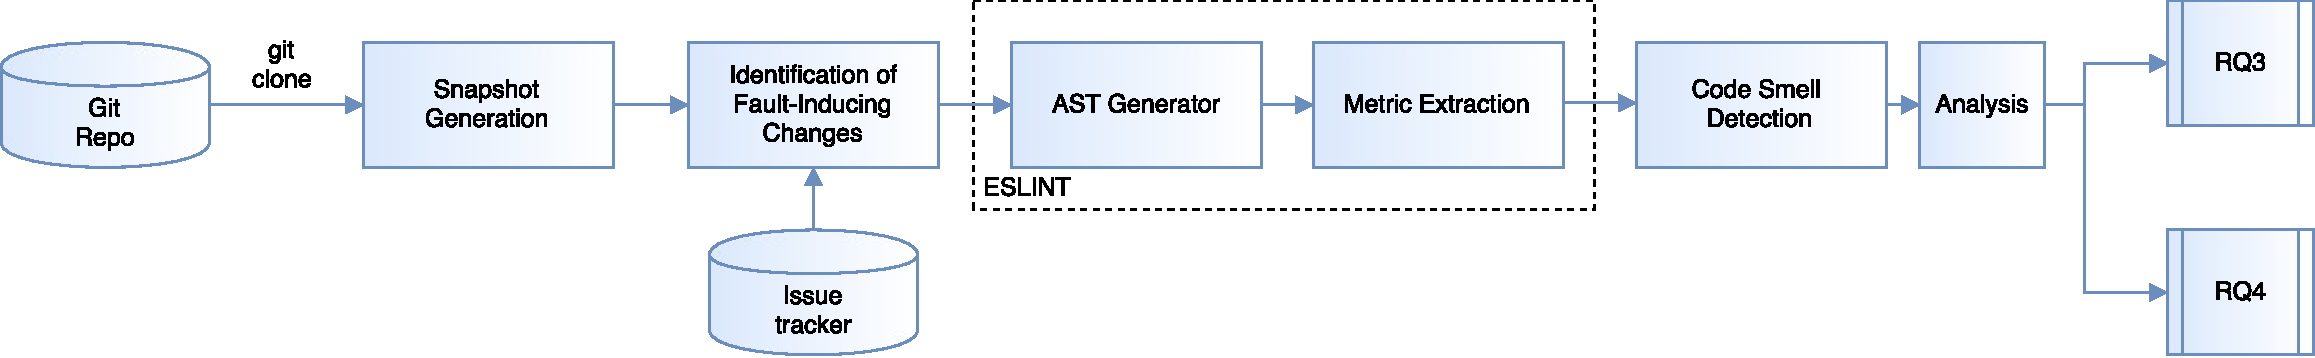
\includegraphics[scale=0.45]{pdfs/total.pdf}
	\caption{Overview of our approach to answer RQ1 and RQ2.}
\label{process}
\vspace{-15pt}
\end{figure*}

\begin{figure*}[t]
	\captionsetup{font=small}
	\centering%
	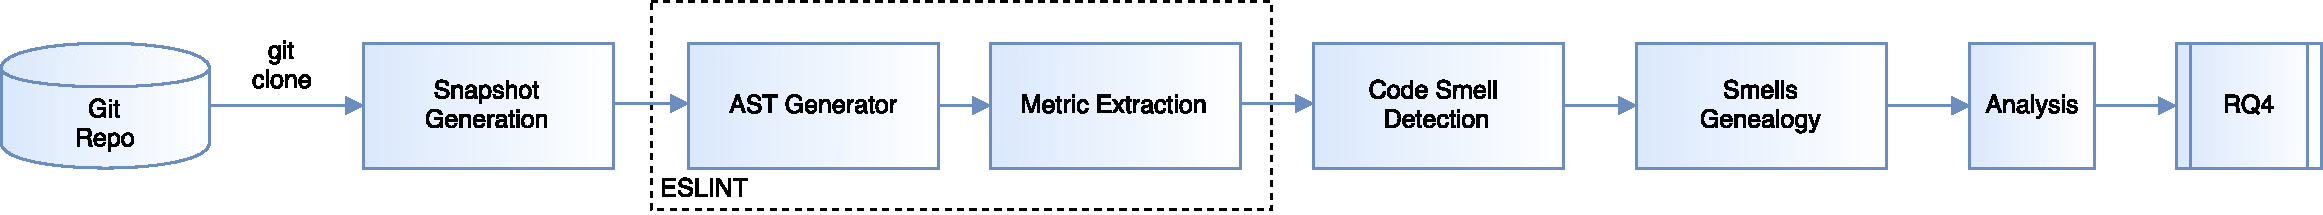
\includegraphics[scale=0.45]{pdfs/total3.pdf}
	\caption{Overview of our approach to answer RQ3.}
	\label{process3}
	\vspace{-15pt}
\end{figure*}

\mytitle{Snapshot Generation} Since all the fifteen studied systems are hosted on Github, at the first step, the framework performs a \texttt{git clone} to get a copy of a system's repository locally. It then generates the list of all the commits and uses it to create snapshots of the system that would be used to perform analysis at commits level.

\mytitle{Identification of Fault-Inducing Changes} Our studied systems use Github as their issue tracker and we use Github APIs to get the list of all the resolved issues on the systems. We leverage the SZZ algorithm~\cite{sliwerski2005changes} to detect changes that introduced faults. We first identify fault-fixing commits using the heuristic proposed by Fischer et al.~\cite{fischer2003populating}, which consists in using regular expressions to detect bug IDs from the studied commit messages. Next, we extract the modified files of each fault-fixing commit through the following Git command:\\

\texttt{git log [commit-id] -n 1 {-{}-}name-status}\\

\noindent
We only take modified JavaScript files into account. Given each file $F$ in a commit $C$, we extract $C$'s parent commit $C'$. Then, we use Git's \texttt{diff} command to extract $F$'s deleted lines. We apply Git's \texttt{blame} command to identify commits that introduced these deleted lines, noted as the ``candidate faulty changes''. We eliminate the commits that only changed blank and comment lines. Then, we filter the commits that were submitted after their corresponding bugs' creation date. {\color{blue}Considering the file $F$ in a fault-fixing commit and its commit that introduced faults, we use again Git's \texttt{diff} command to extract $F$'s changes between both commits, in order to retrieve the ``candidate fault lines'' (useful for our line grain analysis). For the next step, we use UglifyJS\footnote{https://github.com/mishoo/UglifyJS} to get an $F$'s Abstract Syntax Tree (AST) that gives the dependencies of all $F$'s variables, objects and functions (which means their declaration and use lines). We then match $F$'s dependencies with the ``candidate fault lines'' to extend them: given an $F$'s element (variable, object, or function), if one of its declaration or use lines is found into the ``candidate fault lines'', then we add these declaration and use lines to the ``candidate fault lines''. We finally obtain the ``extended candidate fault lines'' (usefull for our line grain analysis including dependencies).
}

\mytitle{AST Generation and Metric Extraction} To automatically detect code smells in the source code, we first extract the Abstract Syntax Tree from the code. AST are being used to parse a source code and generate a tree structure that can be traversed and analyzed programmatically. ASTs are widely used by researchers to analyze the structure of the source code \cite{neamtiu2005understanding, baxter1998clone, pfenning1988higher}.
We used ESLint\footnote{http://eslint.org/} which is a popular and open source lint utility for JavaScript as the core of our framework. Linting tools are widely used in programming to flag the potential non-portable parts of the code by statically analyzing them. ESLint is being used in production in many companies like Facebook, Paypal, Airbnb, etc. ESLint uses espree\footnote{https://github.com/eslint/espree} internally to parse JavaScript source codes and extracts Abstract Source Trees based on the specs\footnote{https://github.com/estree/estree}. ESLint itself provides an extensible environment for developers to develop their own plugins to extract custom information from the source code. We developed our own plugins and modified ESLint built-in plugins to traverse the source tree generated by ESLint to extract and store the information related to our set of code smells described in section \ref{sec:background}. Table~\ref{smellmetric} summarizes all the metrics our framework reports for each type of code smell.

{\color{blue}
\mytitle{Smells Genealogy} Thanks to our previous extraction methods, we easily get, for each Javascript file of a project, the history of the commits that modified those files. Given the history $H$ of a JavaScript file $F$, we identifiy and track $F$'s smells through each commit of $H$. Given two consecutive commits $C1$ and $C2$ of $H$: if one smell appears in $C2$ (and not in $C1$), we consider it as a new smell and keep its date of creation ($C2$'s date); if one smell disappears in $C2$ (and was present in $C1$), we consider it was killed, and keep its date of destruction ($C2$'s date). If a smell if never killed (present in the last commit of $H$), we consider its presence until the last project's commit. To measure the similarity degree between two smells, they first need to be from the same smell type, and then we use SequenceMatcher\footnote{https://docs.python.org/2/library/difflib.html} from difflib (a Python library) that gives us a number between 0 and 1 as a similarity degree (1: both smells are the same; 0: they are totally different). We consider two smells as the same if they are from the same smell type (among the 12 studied), and if their similarity degree is greater than 0.7. If one smell of $C1$ gets a similarity degree greater than 0.7 with two smells of $C2$, we keep the maximum in account. We tried our survival analysis of smells with different thresholds of similarity degree (0.8 and 0.9), but we observe no significant difference with the use of 0.7 threshold.
}

\begin{table*}[!htbp]
\scriptsize
\centering
\caption{Metrics computed for each type of code smell.}
\label{smellmetric}
\begin{tabular}{l|l|l}
\hline
Smell Type                           & Type    & Metric                                                                                                  \\ \hline
Lengthy Lines                        & Number  & The number of characters per line considering the exceptions described in section \ref{sec:background}. \\ \hline
Chained Methods                      & Number  & The number chained methods in each chaining pattern.                                               \\ \hline
Long Parameter List                  & Number  & The number of parameters of each function in source code.                                               \\ \hline
Nested Callbacks                     & Number  & The number of nested functions present in the implementation of each function.                          \\ \hline
Variable Re-assign                   & Boolean & The uniqueness of variables in same scope.                                                              \\ \hline
Assignment in Conditional Statements & Boolean & The presence of assignment operator in conditional statements.                                          \\ \hline
Complex code                         & Number  & The cylcomatic complexity value of each function defined in the source code.                            \\ \hline
Extra Bind                           & Boolean & Whether a function is explicitly bound to a context while not using the context.                        \\ \hline
This Assign                          & Boolean & Whether \texttt{this} is assigned to another variable in a function.                                    \\ \hline
Long Methods                         & Number  & The number of statements in each function.                                                              \\ \hline
Complex Switch Case                  & Number  & The number of case statements in each switch-case block in the source code.                             \\ \hline
Depth                                & Number  & The maximum number of nested blocks in each function.                                                   \\ \hline
\end{tabular}
\vspace{-15pt}
\end{table*}

\mytitle{Code Smell Detection} Among of 12 metric values reported by our framework, 4 are boolean. The boolean metrics concern \emph{This Assign}, \emph{Extra Bind}, \emph{Assignment in Conditional Statements}, and \emph{Variable Re-assign} smells. The 8 remaining metrics are integers. To identify code smells using the metric values provided by our framework, we follow the same approach as previous works~\cite{saboury2017empirical,marinescu2004detection, mazinanian2016migrating}, defining threshold values above which files should be considered as having the code smell. We define the thresholds relative to the systems using Box-plot analysis. We chose to define threshold values relative to the projects because design rules and programming styles can vary from one project to another, and hence it is important to compare the characteristics of files in the context of the project. For each system, we obtain the threshold values as follows. We examined the distribution of the metrics and observed a big gap around the first 70\% of the data and the top 10\%. Hence, we decided to consider files with metric values in the top 10\% as containing the code smell. For files that contain multiple functions, we aggregated the metric values reported for each functions using the maximum to obtain a single value characterizing the file. %of the metric values reported for each function contained in the file to obtain a metric value characterizing the file.

%aformentioned In order to convert those numeric values into boolean which indicate the presence of a type of smell, we used a statistical approach to define the threshold . Since the culture, style guide and design rules could be different from a project to another, we defined the threshold specifically for each project in our case study.
%
%To define the threshold, we first removed the top 1\% of the data to remove extreme cases. By looking at the distribution of the numeric values of extracted metrics, for most of the metrics we saw there is a big gap around the first 70\% of the data and the top 10\%. So we considered the top 10\% of each metric as smelly codes. To analyze the sensitivity of the threshold to the result, we rerun our analysis with the threshold values of top 20\% and top 30\% as well and we observed no significant difference.
%Also as files could contain multiple functions and so multiple smelly parts, our framework could extract multiple values for each file for each numeric metric. To reduce this list of values to a single number, we get the maximum value of the list and associated that with the file.
%
%\section{Code Smells}\label{smells}
%Code smells are the results of bad design choices. They are referred to the structural characteristics in software code which could make the software harder to maintain or evolve \cite{fontana2012automatic}. Code smells usually the starting point of re-factoring \cite{fontana2012automatic, hamza2008code, fard2013jsnose}.

%\mytitle{Analysis}
%At the end, we feed the data to our R scripts to generate the result. We wrapped the R scripts into our framework to automate the whole process. In the following %section we will discuss about our analysis approach. 

\subsection{Analysis}\label{survival}
To assess the impact of code smells on the fault-proneness {\color{blue}of JavaScript files, or to assess the smells survival over project lifetime,} we perform survival analysis, comparing the time until {\color{blue}a fault occurrence}, in files containing code smells and files without code smells, {\color{blue}or comparing the time until a type smell occurrence in files containing code smells, for each of the 12 studied type smell.}\\
\textbf{Survival analysis} is used to model the time until the occurrence of a well-defined event~\cite{fox2010r}. One of the most popular models for survival analysis is the Cox Proportional Hazards (Cox) model. A Cox hazard model is able to model the instantaneous hazard of the occurrence of an event as a function of a number of independent variables~\cite{koru2008theory}~\cite{singer2003applied}. Particularly, Cox models aim to model how long subjects under observation can \textsl{survive} before the occurrence of an event of interest (a fault occurrence in our case) ~\cite{singer2003applied}~\cite{selim2010studying}.

Survival models were first introduced in demography and actuarial sciences~\cite{Westergaard}. Recently, researchers have started applying them to problems in the domain of Software Engineering. For example, Selim et al.~\cite{selim2010studying} used the Cox model to investigate characteristics of cloned code that are related to the occurrence of faults. Koru et al.~\cite{koru2007modeling} also used Cox models to analyze faults in software systems. %formulated the modeling by using Cox in order to find the effect of size on the defects.
In Cox models, the hazard of a fault occurrence at a time t is modeled by the following function:

\begin{equation}\label{eq1}
\lambda_{i}(t) = \lambda_{0}(t)* e ^ {\beta*{F_{i}}(t)}
\end{equation}

If we take log from both sides, we obtain:

\begin{equation}\label{eq2}
log(\lambda_{i}(t)) = log(\lambda_{0}(t)) + {\beta_{1}*{f_{i1}}(t)} + ... + {\beta_{n}*{f_{in}}(t)}
\end{equation}

Where:
\begin{itemize}
	\item ${F_{i}}(t)$ is the time-dependent covariates of observation $i$ at the time $t$.
	\item $\beta$ is the coefficient of covariates in the function ${F_{i}}(t)$.	
	\item $\lambda_0$ is the baseline hazard.
	\item $n$ is the number of covariates.
\end{itemize}

When all the covariates have no effect on the hazard, the baseline hazard can be considered as the hazard of occurrence of the event (\ie{} a fault). The baseline hazard would be omitted when formulating the relative hazard between two files (in our case) at a specific time, as shown in the following Equation~\ref{eq3}.

\begin{equation}\label{eq3}
\lambda_{i}(t) \slash \lambda_{j}(t) = e ^ {\beta*{(f_{i}(t) - f_{j}(t))}}
\end{equation}

The proportional hazard model assumes that changing each covariate has the effect of multiplying the hazard rate by a constant.

%It is obvious that the relative hazard has nothing to do with the baseline hazard. This is called the proportional hazard assumption.

\textbf{Link function}. As Equation~\ref{eq2} shows, the log of the hazard is a linear function of the log of the baseline hazard and all the other covariates. In order to build a Cox proportional model, a linear relationship should be available between the log hazard and the covariates~\cite{therneau2000modeling}. Link functions are used to transform the covariates to a new scale if such relationship does not exist. Determining an appropriate link function for covariates is necessary because it allows changes in the original value of a covariate to influence the log hazard equally. This allows the proportionality assumption to be valid and applicable~\cite{therneau2000modeling}.

\textbf{Stratification}. In addition to applying a link function, a stratification is sometimes necessary to preserve the proportionality in Cox hazard models \cite{koru2008theory}. For example, if there is a covariate that needs to be controlled because it is of no interest or secondary, stratification can be used to split the data set so that the influence of more important covariates can be monitored better \cite{koru2008theory}.

\textbf{Model validation}. Since Cox proportional hazard models assume that all covariates are consistent over time and the effect of a covariate does not fluctuate with time, hence, to validate our model, we apply a non-proportionality test to ensure that the assumption is satisfied~\cite{therneau2000modeling} \cite{selim2010studying}.

In this paper, we perform our analysis at commit level. For each file, we use Cox proportional hazard models to calculate the risk of a fault occurrence over time, considering a number of independent covariates. We chose Cox proportional hazard model, {\color{blue}as well as our predecessors~\cite{saboury2017empirical},} for the following reasons:\\
(1) In general, not all files in a commit experience a fault. Cox hazard models allow files to remain in the model for the entire observation period, even if they don't experience the event (\ie{} fault occurrence). (2) In Cox hazard models, subjects can be grouped according to a covariate (\eg{} smelly or non-smelly). (3) The characteristics of the subjects might change during the observation period (\eg{} size of code), and (4) Cox hazard models are adapted for events that are recurrent~\cite{therneau2000modeling}, which is important because software modules evolve over time and a file can have multiple faults during its life cycle. 

\section{Case Study Results}\label{sec:case-study}
In this section, we report and discuss the results for each research question. {\color{blue}For each research question, we collect information about smell, fault hazard, and vulnerability codes of JavaScript files of the studied systems, and more specifically those which end with the \textsl{.js} extension. Also, we don't take in account the JavaScript files with \textsl{.min.js} extension, because they are a minified version of \textsl{.js} files that we already keep in our study. In this way, we avoid redundancy in our analyzes.}

\subsection*{(RQ1) Is the risk of fault higher in files with code smells in comparison with those without code smell?}

%\textbf{Motivation}. Code smells are poor solutions in software design and implementation problems. Previous studies such as Jaafar et al.~\cite{jaafar2013mining} has shown that the fault-proneness of modules are significantly different between implementations with code smells and implementations without them. As stated by ~\cite{jaafar2013mining}: ``classes having dependencies with anti-patterns are more fault-prone than others". However, their study has been done on Java software systems. To the best of our knowledge, less is known on the code smells of JavaScript. Hence, in this research question we aim to explore how code smells affect the reliability of a software developed in JavaScript.

%This knowledge helps software practitioners plan to detect the code smells as much early as possible in the very beginning phase of software development before the code base gets %bigger.%

\begin{figure*}[t]
\centering%
\subfigure[express.js]{%
{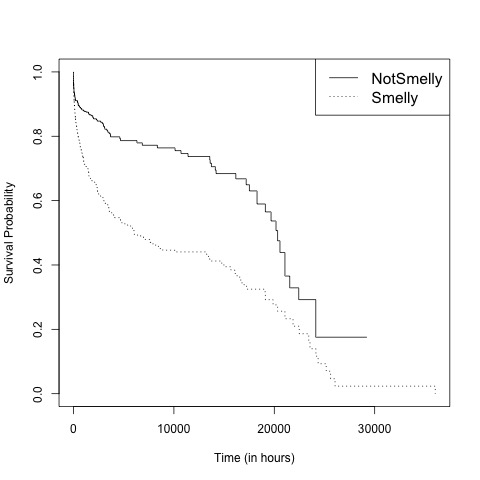
\epsfig{file = pdfs/Express_bugs_smells_file-grain_rplot.jpg, width = 3.5cm}}%
}
\subfigure[request.js]{%
{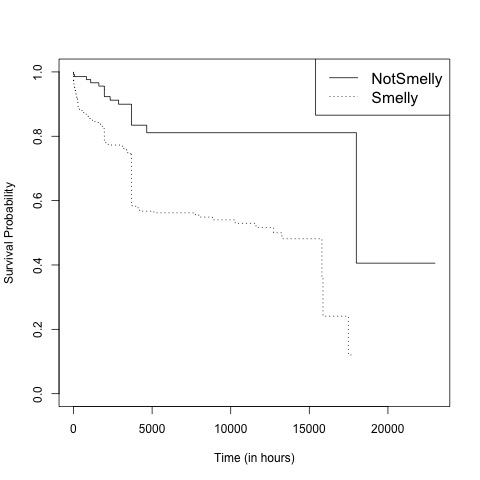
\epsfig{file = pdfs/Request_bugs_smells_file-grain_rplot.jpg, width = 3.5cm}}%
}
\subfigure[less.js]{%
{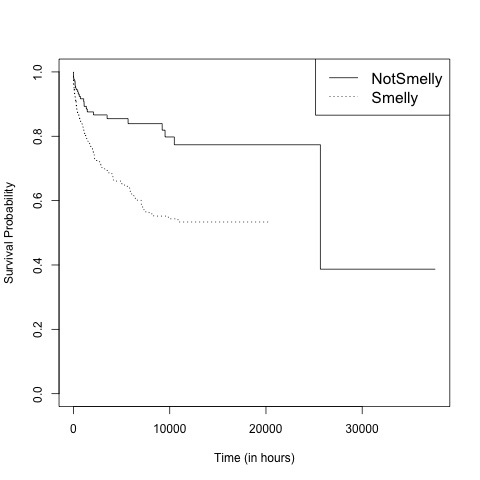
\epsfig{file = pdfs/Less_bugs_smells_file-grain_rplot.jpg, width = 3.5cm}}%
}
\subfigure[grunt.js]{%
{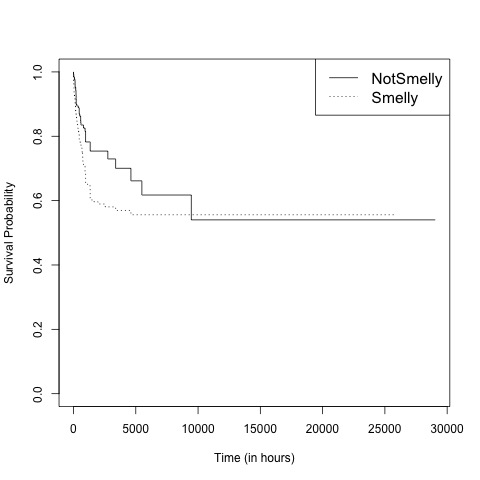
\epsfig{file = pdfs/Grunt_bugs_smells_file-grain_rplot.jpg, width = 3.5cm}}%
}
\subfigure[bower.js]{%
{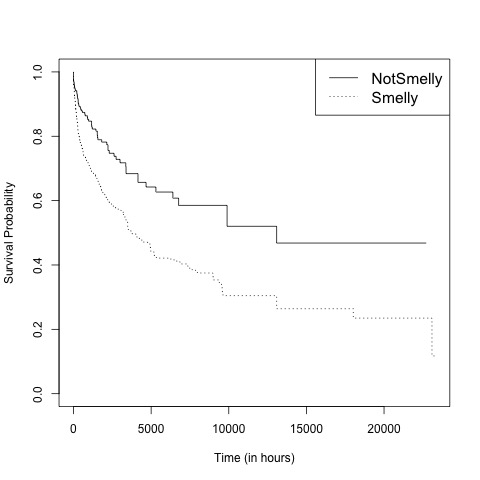
\epsfig{file = pdfs/Bower_bugs_smells_file-grain_rplot.jpg, width = 3.5cm}}%
}
\subfigure[jquery.js]{%
	{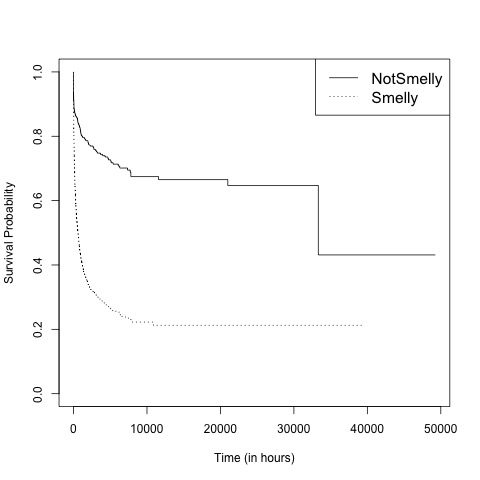
\epsfig{file = pdfs/Jquery_bugs_smells_file-grain_rplot.jpg, width = 3.5cm}}%
}
\subfigure[hexo.js]{%
	{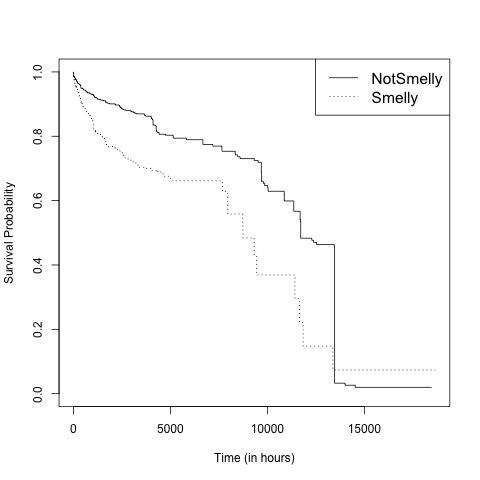
\epsfig{file = pdfs/Hexo_bugs_smells_file-grain_rplot.jpg, width = 3.5cm}}%
}
\subfigure[leaflet.js]{%
	{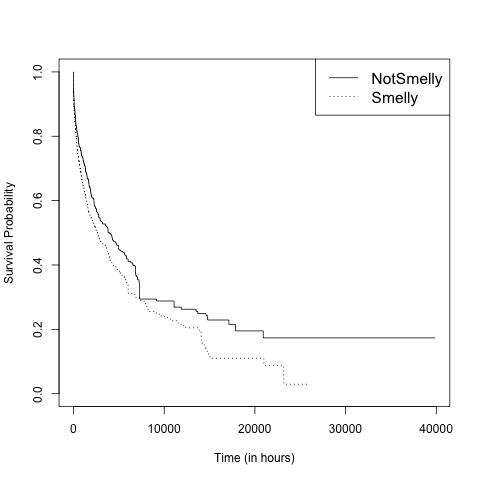
\epsfig{file = pdfs/Leaflet_bugs_smells_file-grain_rplot.jpg, width = 3.5cm}}%
}
\subfigure[ramda.js]{%
	{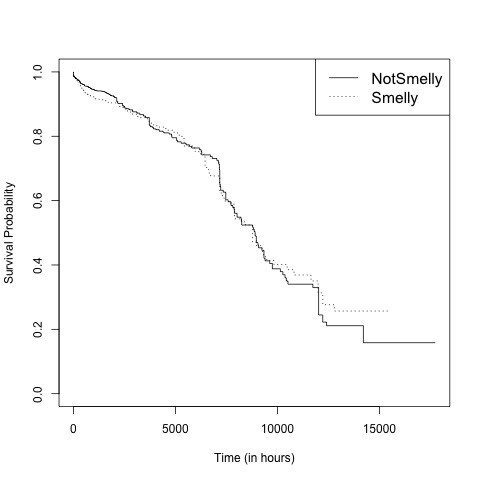
\epsfig{file = pdfs/Ramda_bugs_smells_file-grain_rplot.jpg, width = 3.5cm}}%
}
\subfigure[chart.js]{%
	{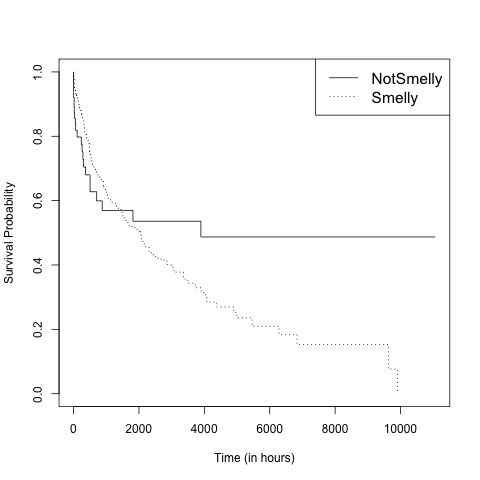
\epsfig{file = pdfs/Chart_bugs_smells_file-grain_rplot.jpg, width = 3.5cm}}%
}
\subfigure[riot.js]{%
	{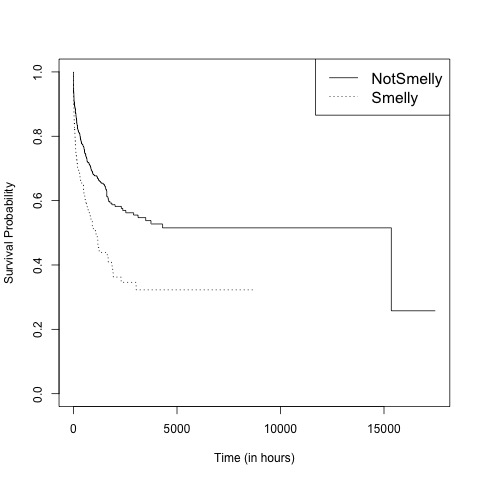
\epsfig{file = pdfs/Riot_bugs_smells_file-grain_rplot.jpg, width = 3.5cm}}%
}
\subfigure[vue.js]{%
	{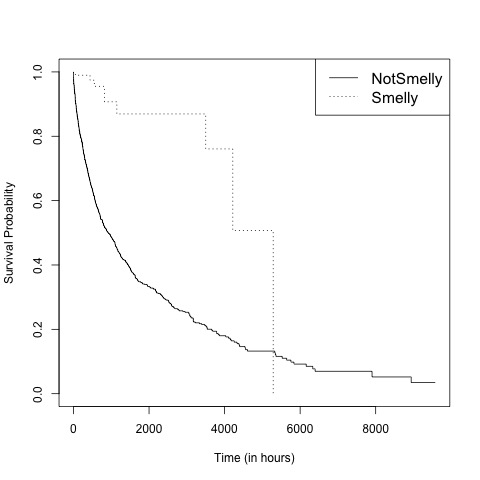
\epsfig{file = pdfs/Vue_bugs_smells_file-grain_rplot.jpg, width = 3.5cm}}%
}
\subfigure[moment.js]{%
	{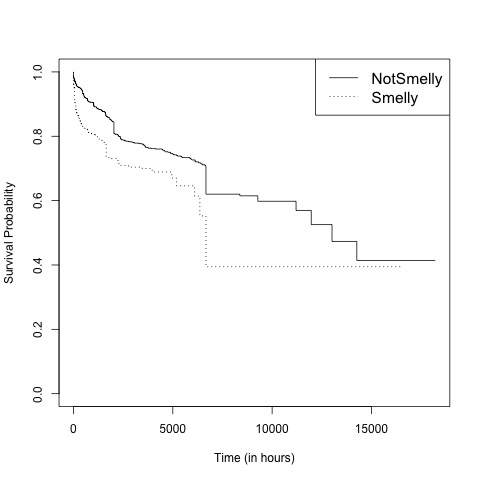
\epsfig{file = pdfs/Moment_bugs_smells_file-grain_rplot.jpg, width = 3.5cm}}%
}
\subfigure[webpack.js]{%
	{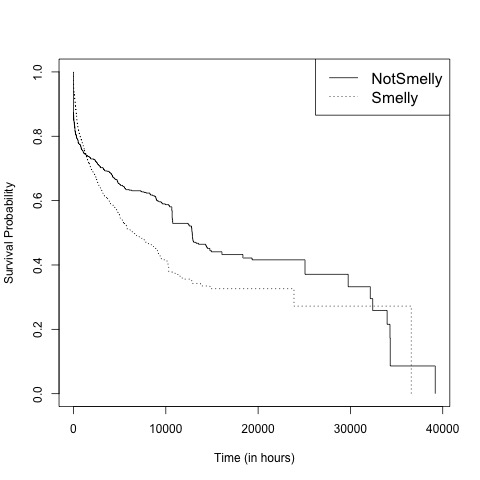
\epsfig{file = pdfs/Webpack_bugs_smells_file-grain_rplot.jpg, width = 3.5cm}}%
}
\subfigure[webtorrent.js]{%
	{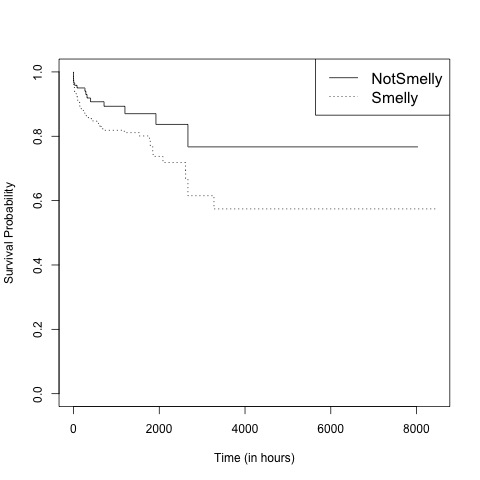
\epsfig{file = pdfs/Webtorrent_bugs_smells_file-grain_rplot.jpg, width = 3.5cm}}%
}
\caption{Survival probability trends of smelly codes vs. non-smelly codes in our fifteen JavaScript projects with the file grain approach (hazard study).\vspace{-10pt}}
\label{rq1}
\end{figure*}

\begin{table*}[t]
	\centering
	\scriptsize
	\caption{Fault hazard ratios for each project with the line grain approach. $exp(coef)$ values means higher hazard rates.}
	\label{hazardlinegrain}
	\begin{tabular}{l|l|l|l}
		\hline
		module & $exp(coef)$ & $p$-value (Cox hazard model) & $p$-value (Proportional hazards assumption)     \\ \hline
		express  & 1.341 & 0.002 & 0.192 \\ \hline
		request  & 2.538 & 0.028e-2 & 0.602 \\ \hline
		less  & 1.791 & 0.003 & 0.419 \\ \hline
		bower	 & 1.321 & 0.027 & 0.982 \\ \hline
		grunt    & 0.594 & 0.005 & 0.019 \\ \hline
		jquery	 & 3.436 & 0 & 1.197e-8 \\ \hline
		vue   & 0.062 & 0.011e-9 & 0.843 \\ \hline
		ramda 	 & 0.460 & 0.01e-8 & 3.691e-5 \\ \hline
		leaflet	 & 0.725 & 0.088e-4 & 0.739 \\ \hline
		hexo	 & 1.199 & 0.077 & 0.945 \\ \hline
		chart	 & 0.711 & 0.136 & 1.46e-9 \\ \hline
		webpack	 & 0.603 & 0 & 0 \\ \hline
		webtorrent & 1.222 & 0.047e-9 & 0.045 \\ \hline
		moment	 & 0.941 & 0.401 & 5.046e-5 \\ \hline
		riot	 & 1.047 & 0.586 & 0.797 \\ \hline
	\end{tabular}

\end{table*}

\begin{figure*}[t]
	\centering%
	\subfigure[express.js]{%
		{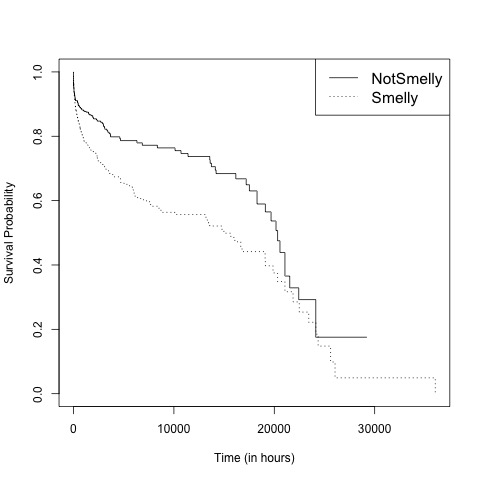
\epsfig{file = pdfs/Express_bugs_smells_line-grain_large_rplot.jpg, width = 3.5cm}}%
	}
	\subfigure[request.js]{%
		{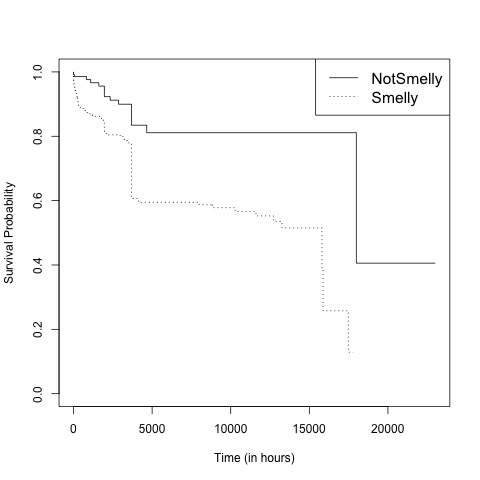
\epsfig{file = pdfs/Request_bugs_smells_line-grain_large_rplot.jpg, width = 3.5cm}}%
	}
	\subfigure[less.js]{%
		{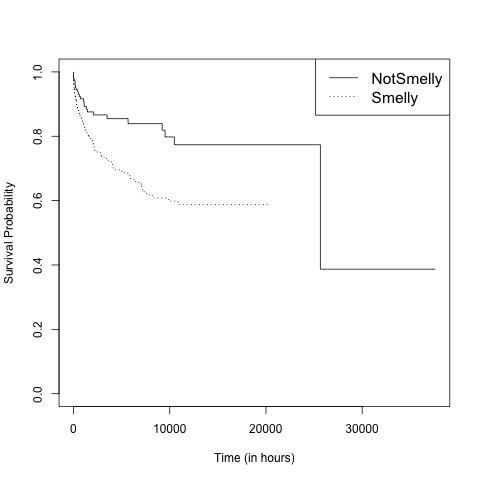
\epsfig{file = pdfs/Less_bugs_smells_line-grain_large_rplot.jpg, width = 3.5cm}}%
	}
	\subfigure[grunt.js]{%
		{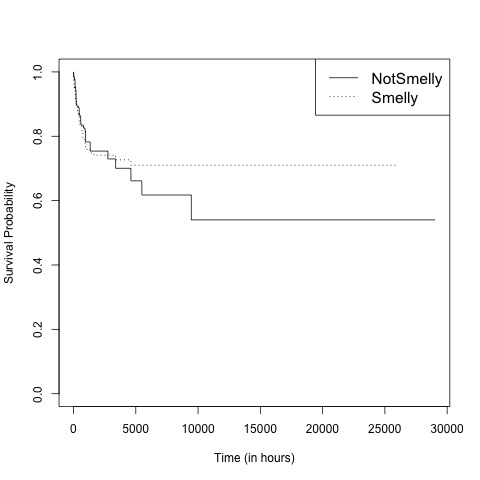
\epsfig{file = pdfs/Grunt_bugs_smells_line-grain_large_rplot.jpg, width = 3.5cm}}%
	}
	\subfigure[bower.js]{%
		{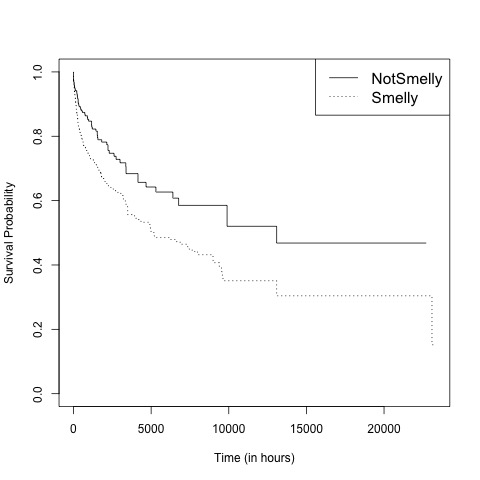
\epsfig{file = pdfs/Bower_bugs_smells_line-grain_large_rplot.jpg, width = 3.5cm}}%
	}
	\subfigure[jquery.js]{%
		{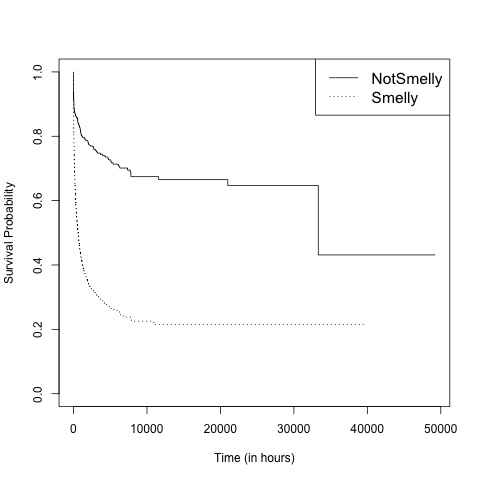
\epsfig{file = pdfs/Jquery_bugs_smells_line-grain_large_rplot.jpg, width = 3.5cm}}%
	}
	\subfigure[hexo.js]{%
		{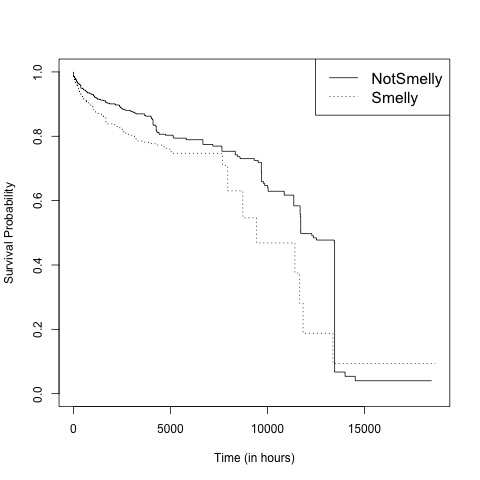
\epsfig{file = pdfs/Hexo_bugs_smells_line-grain_large_rplot.jpg, width = 3.5cm}}%
	}
	\subfigure[leaflet.js]{%
		{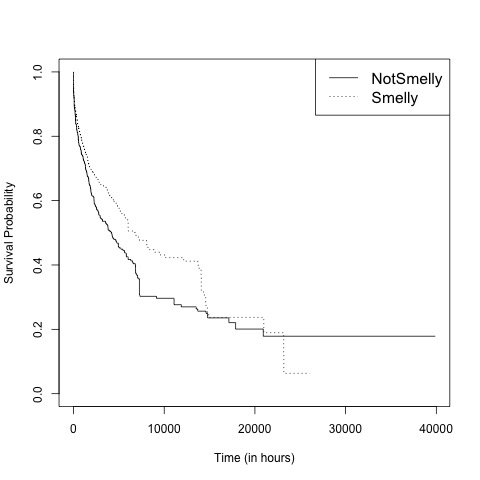
\epsfig{file = pdfs/Leaflet_bugs_smells_line-grain_large_rplot.jpg, width = 3.5cm}}%
	}
	\subfigure[ramda.js]{%
		{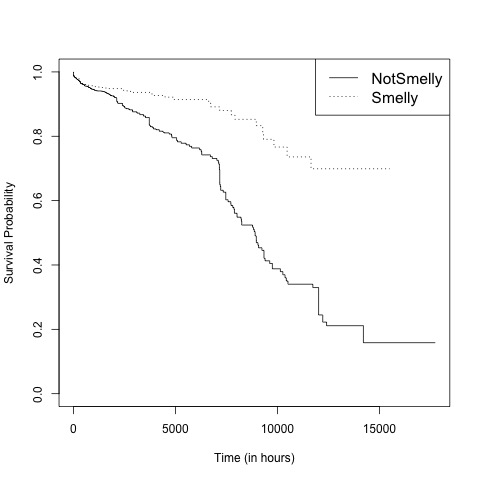
\epsfig{file = pdfs/Ramda_bugs_smells_line-grain_large_rplot.jpg, width = 3.5cm}}%
	}
	\subfigure[chart.js]{%
		{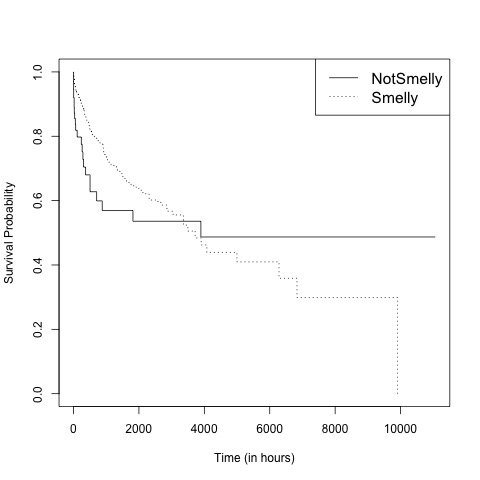
\epsfig{file = pdfs/Chart_bugs_smells_line-grain_large_rplot.jpg, width = 3.5cm}}%
	}
	\subfigure[riot.js]{%
		{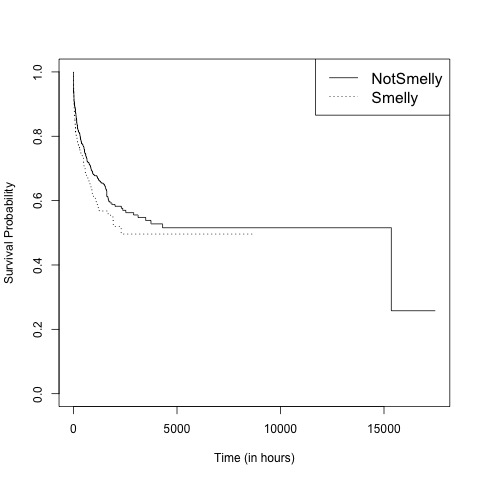
\epsfig{file = pdfs/Riot_bugs_smells_line-grain_large_rplot.jpg, width = 3.5cm}}%
	}
	\subfigure[vue.js]{%
		{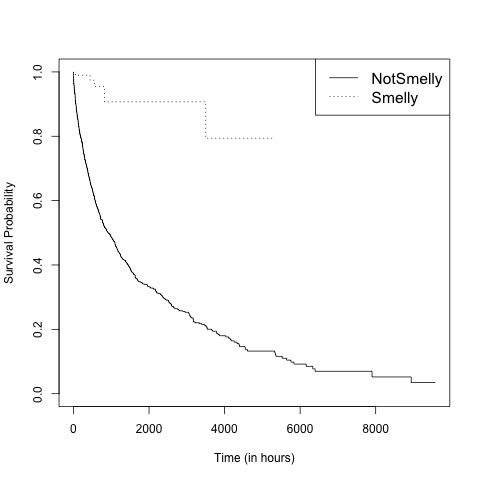
\epsfig{file = pdfs/Vue_bugs_smells_line-grain_large_rplot.jpg, width = 3.5cm}}%
	}
	\subfigure[moment.js]{%
		{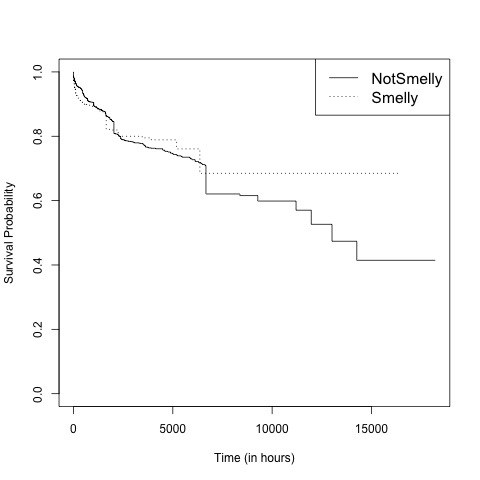
\epsfig{file = pdfs/Moment_bugs_smells_line-grain_large_rplot.jpg, width = 3.5cm}}%
	}
	\subfigure[webpack.js]{%
		{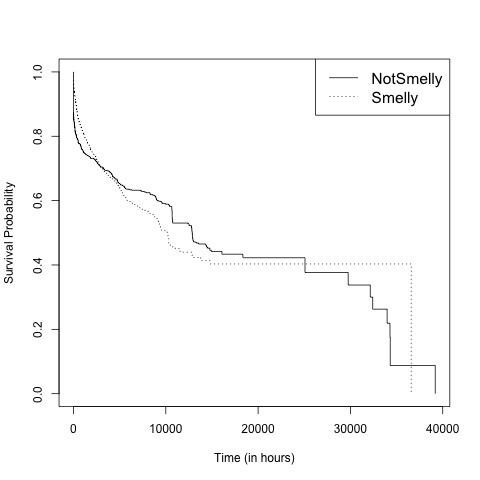
\epsfig{file = pdfs/Webpack_bugs_smells_line-grain_large_rplot.jpg, width = 3.5cm}}%
	}
	\subfigure[webtorrent.js]{%
		{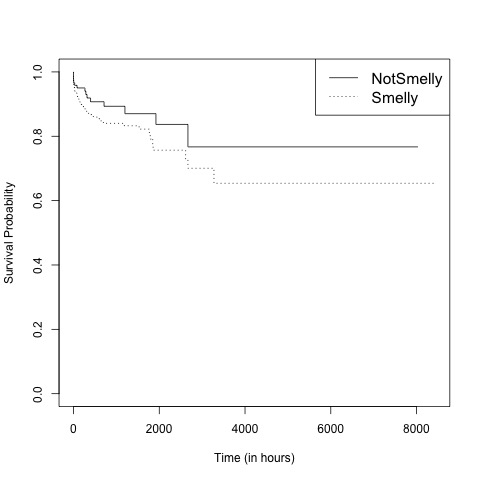
\epsfig{file = pdfs/Webtorrent_bugs_smells_line-grain_large_rplot.jpg, width = 3.5cm}}%
	}
	\caption{Survival probability trends of smelly codes vs. non-smelly codes in our fifteen JavaScript projects with the line grain including dependencies approach.\vspace{-10pt}}
	\label{rq1-2}
\end{figure*}

\textbf{Approach}. We use our framework described in Section~\ref{extraction} {\color{blue}(Figure~\ref{process})} to collect information about the occurrence of the 12 studied code smells in our {\color{blue}fifteen} subject systems. %fetch all the data considering all 12 types of code smells.
For each file and for each revision $r$ (\ie{} corresponding to a commit), we also compute the following metrics:
\begin{itemize}
\item \textbf{Time:} the number of hours between the previous revision of the file and the revision $r$. 
We set the time of the first revision to zero.
\item \textbf{Smelly:} this is our covariate of interest. It takes the value $1$ if the revision $r$ of the file contains a code smell and $0$ if it doesn't contain any of the 12 studied code smells. 
\item \textbf{Event:} {\color{blue}for the file grain approach,} this metric takes the value $1$ if the revision $r$ is a fault-fixing change and $0$ otherwise. We use the SZZ algorithm to insure that the file contained a code smell when the fault was introduced. {\color{blue}For the line grain and line grain including dependencies approaches, this metric takes the value $1$ if the revision $r$ is a fault-fixing change and if there is at least one match between the fault lines and the smell lines, and $0$ otherwise. Indeed, if there is no matching, we consider that the fault-fixing change doesn't fix any code smells.}
\end{itemize}

Using the smelly metric, we divide our dataset in two groups: one group containing files with code smells (\ie{} smelly = 1) and another group containing files without any of the 12 studied code smells (\ie{} smelly = 0). For each group we create an individual Cox hazard model. In each group, the covariate of interest (\ie{} smelly) is a constant function (with value either 1 or 0), hence, there is no need for a link function to establish a linear relationship between this covariate and our event of interest, \ie{} the occurrence of a fault. We use the \textsl{survfit} and \textsl{coxph} functions from R~\cite{rPackage} to analyze our Cox hazard models.

In addition to building Cox hazard models, we test the following null hypothesis: \emph{$H^{1}_{0}$: There is no difference between the probability of a fault occurrence in a file containing code smells and a file without code smells}. We use the \textsl{log-rank} test (which compares the survival distributions of two samples), to accept or refute this null hypothesis.

\textbf{Findings}. {\color{blue}File grain} results presented in Figure~\ref{rq1} show that files containing code smells experience faults faster than files without code smells. {\color{blue}Table~\ref{hazardlinegrain} (line grain results) and Figure~\ref{rq1-2} (line grain including dependencies results) show the same minimized but still acceptable observation, wich means files containing code smells experience faults faster than files without code smells.} The $Y$-axis in Figure~\ref{rq1} {\color{blue}and Figure~\ref{rq1-2}} represents the probability of a file \emph{surviving} a fault occurrence. Hence a low value on the $Y$-axis means a low \emph{survival} rate (\ie{} a high hazard or high risk of fault occurrence).  
For all {\color{blue}fifteen} projects, {\color{blue}and for each approach (file grain, line grain, and line grain including dependencies),} we calculated relative hazard rates (using Equation~\ref{eq3} from Section~\ref{survival}) between files containing code smells and files without code smells. Results show that, on average, files without code smells have hazard rates {\color{blue}76\% lower than files with code smells in our file grain analysis, 20\% lower in our line grain analysis, and 38\% lower in our line grain analysis including dependencies. It is normal to see this pourcentage decreasing in line grain approach, because we add an additional matching condition to set the \emph{event} to $1$. Between the line grain and the line grain including dependencies analyzes, this pourcentage increases due to the increasing of the fault lines number considering during the compute of \emph{event}.} We performed a \textsl{log-rank} test comparing the survival distributions of files containing code smells and files without any of the studied code smells and obtained $p$-values lower than $0.05$ for {\color{blue}most of the fifteen} studied systems. Hence, we reject $H^{1}_{0}$.
Since our detection of code smells depends on our selected threshold value (\ie{} the top 10\% value chosen in Section~\ref{extraction}), we conducted a sensitivity analysis to assess the potential impact of this threshold selection on our result. More specifically, we rerun all our analysis with threshold values at top 20\% and top 30\%. We observed no significant differences in the results. Hence, we conclude that:

\hypobox{JavaScript files without code smells have hazard rates {\color{blue}76\%} lower than JavaScript files with code smells {\color{blue}in the file grain approach}, and this difference is statistically significant. {\color{blue}Plus, this difference still remains significant in the line grain including dependencies approach, because hazard rates reach 38\%.}}


\begin{figure}[t]
\centering
\captionsetup{font=small}
\minipage{0.2\textwidth}
  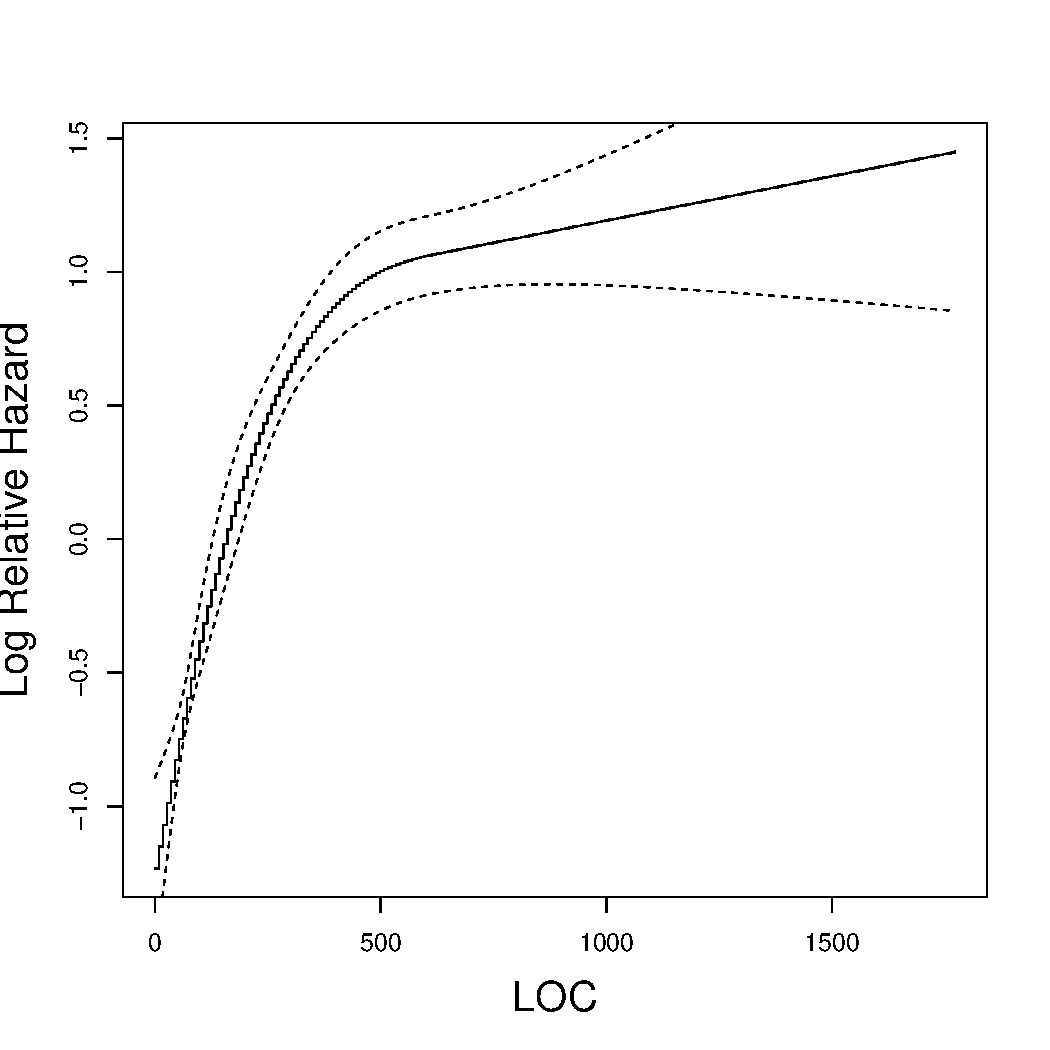
\includegraphics[width=\linewidth]{pdfs/linkExpress.pdf}
\endminipage
\minipage{0.2\textwidth}
  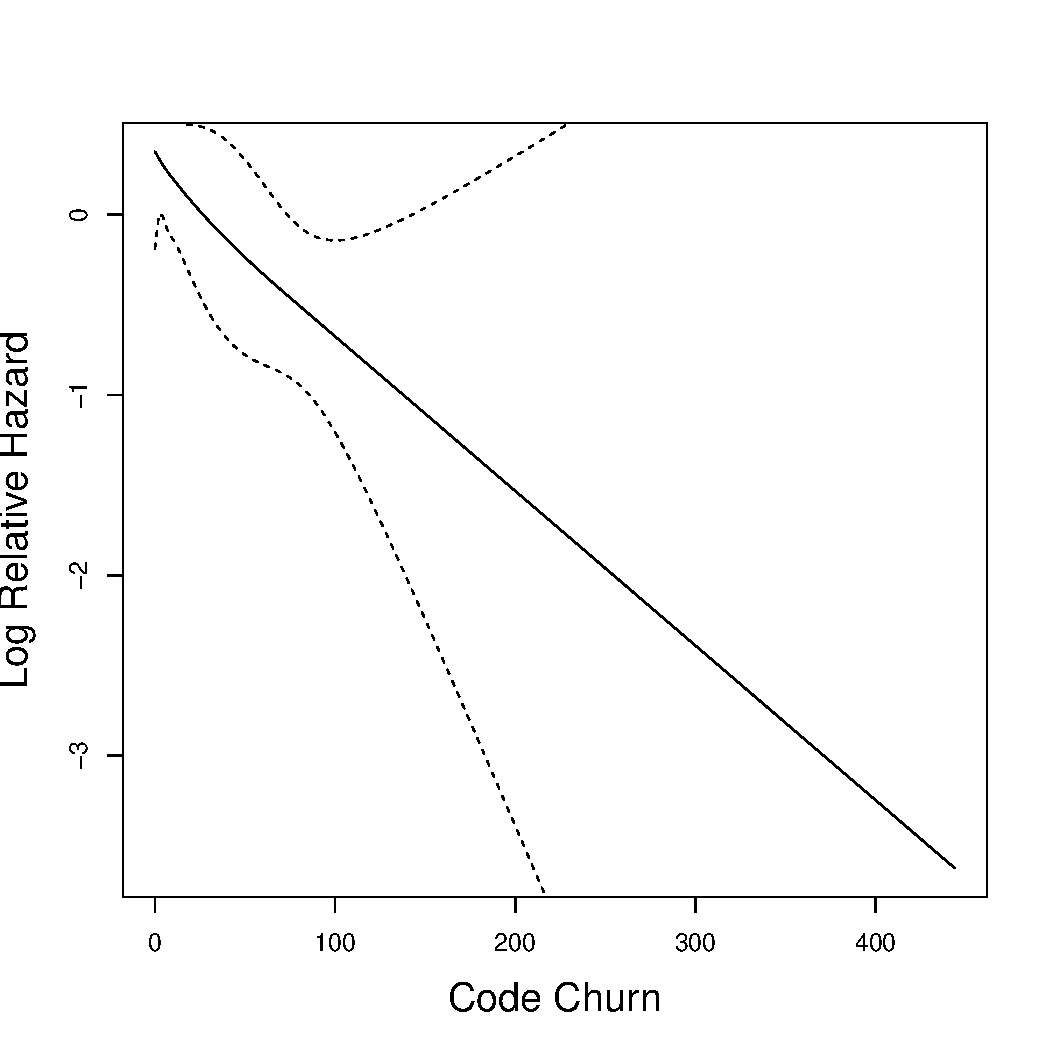
\includegraphics[width=\linewidth]{pdfs/linkTotalChurnGrunt.pdf}
\endminipage
\caption{Determining a link function for express.js (left figure) and grunt.js (right figure) modules for two covariates: LOC and Code Churn respectively.\vspace{-10pt}}\label{link}
\end{figure}

\subsection*{(RQ2) Are JavaScript files with code smells equally fault-prone?}

%\begin{table*}[t]
%\centering%
%\caption{Covariates coeffiecients on the defects. Higher exp(coef) means higher hazard rate.}
%\begin{tabular}{c|c|c|c|c|c|c}
%\hline
%module & covariate & exp(coef) & se(coef) & z & p & Non-proportionality test (p-value) \\ \hline
%\multirow{3}{*}{express} & No.Previous-Bugs & 1.01842956 & 0.00300334 & 6.08 & 0.0000000012 & 0.887 \\ \cline{2-7}
% & cond.assign & 1.55093782 & 0.14811000 & 2.96 & 0.0030 & 0.561 \\ \cline{2-7}
% & LOC & 1.00111187 & 0.00019567 & 5.68 & 0.0000000135 & 0.382 \\ \hline
%\multirow{2}{*}{grunt} & cond.assign & 2.36768081 & 0.24248431 & 3.55 & 0.00038 & 0.2237 \\ \cline{2-7}
% & nested.callbacks & 3.13565940 & 0.41026000 & 2.79 & 0.00534 & 0.8147 \\ \hline
%\multirow{3}{*}{bower} & No.Previous-Bugs & 1.025646 & 0.007863 & 3.22 & 0.0013 & 0.415 \\ \cline{2-7}
% & max.depth & 9.222632 & 0.452966 & 4.90 & 0.00000094 & 0.960 \\ \cline{2-7}
% & LOC & 1.000643 & 0.000295 & 2.18 & 0.0295 & 0.414 \\ \hline
%\multirow{3}{*}{less} & No.Previous-Bugs & 1.036634202 & 0.003126697 & 11.51 & 0.000002 & 0.739 \\ \cline{2-7}
% & complex.switch.case & 0.484588521 & 0.332039480 & -2.18 & 0.02912 & 0.4177 \\ \cline{2-7}
% & cond.assign & 1.664212015 & 0.131560216 & 3.87 & 0.00011 & 0.9154 \\ \hline
%\multirow{3}{*}{request} & No.Previous-Bugs & 1.0675617 & 0.0218429 & 2.99 & 0.0028 & 0.4074 \\ \cline{2-7}
% & max.depth & 0.1723391 & 0.4346634 & -4.05 & 0.000052 & 0.6207 \\ \cline{2-7}
% & LOC & 1.0009179 & 0.0003798 & 2.42 & 0.0157 & 0.8668 \\ \hline
%\end{tabular}
%\end{table*}

% Please add the following required packages to your document preamble:
% \usepackage{multirow}
%\begin{table*}[t]
%\centering%
%\caption{Covariates coeffiecients on the defects. Higher exp(coef) means higher hazard rate.}
%\begin{tabular}{c|c|c|c|c}
%\hline
%module & covariate & exp(coef) & p & Non-proportionality test (p-value) \\ \hline
%\multirow{3}{*}{express} & No.Previous-Bugs & 1.01842956 & 0.0000000012 & 0.887 \\ \cline{2-5}
% & cond.assign & 1.55093782 & 0.0030 & 0.561 \\ \cline{2-5}
% & LOC & 1.00111187 & 0.0000000135 & 0.382 \\ \hline
%\multirow{2}{*}{grunt} & cond.assign & 2.36768081 & 0.00038 & 0.2237 \\ \cline{2-5}
% & nested.callbacks & 3.13565940 & 0.00534 & 0.8147 \\ \hline
%\multirow{3}{*}{bower} & No.Previous-Bugs & 1.025646 & 0.0013 & 0.415 \\ \cline{2-5}
% & max.depth & 9.222632 & 0.00000094 & 0.960 \\ \cline{2-5}
% & LOC & 1.000643 & 0.0295 & 0.414 \\ \hline
%\multirow{3}{*}{less} & No.Previous-Bugs & 1.036634202 & 0.000002 & 0.739 \\ \cline{2-5}
% & complex.switch.case & 0.484588521 & 0.02912 & 0.4177 \\ \cline{2-5}
% & cond.assign & 1.664212015 & 0.00011 & 0.9154 \\ \hline
%\multirow{3}{*}{request} & No.Previous-Bugs & 1.0675617 & 0.0028 & 0.4074 \\ \cline{2-5}
% & max.depth & 0.1723391 & 0.000052 & 0.6207 \\ \cline{2-5}
% & LOC & 1.0009179 & 0.0157 & 0.8668 \\ \hline
%\end{tabular}
%\end{table*}

% Please add the following required packages to your document preamble:
% \usepackage{multirow}
\begin{table}[t]
\centering
\scriptsize
\caption{Hazard ratios for each type of code smells with file grain approach. Higher $exp(coef)$ values means higher hazard rates.}
\begin{tabular}{c|c|c|p{1.1cm}|p{1.3cm}}
\hline
module & covariate & $exp(coef)$ & $p$-value (Cox hazard model) & $p$-value (Proportional hazards assumption) \\ \hline
\multirow{4}{*}{express}
 & No.Previous-Bugs & 1.031 & 0 & 0.076 \\ \cline{2-5}
 & Long Methods & 3.363 & 0.012e-11 & 0.14 \\ \cline{2-5}
 & Complex Switch Case & 2.528 & 0.043e-8 & 0.322 \\ \cline{2-5}
 & Variable Re-assign & 1.927 & 0.056e-14 & 0.725  \\ \hline
\multirow{4}{*}{grunt} 
 & No.Previous-Bugs & 1.051 & 0.003 & 0.925 \\ \cline{2-5}
 & Nested Callbacks & 3.609 & 0.086e-3 & 0.65 \\ \cline{2-5}
 & Assign. in Cond. State. & 2.008 & 0.004 & 0.707 \\ \cline{2-5}
 & Long Methods & 1.8 & 0.019 & 0.098 \\ \hline
\multirow{5}{*}{bower}
 & No.Previous-Bugs & 1.047 & 0 & 0.596 \\ \cline{2-5}
 & LOC & 1.001 & 0.023e-13 & 0.379 \\ \cline{2-5}
 & Complex Code & 5.778 & 0 & 0.432 \\ \cline{2-5}
 & Long Methods & 3.55 & 0 & 0.525 \\ \cline{2-5}
 & Extra Bind & 3.03 & 0.097e-5 & 0.378 \\ \hline
\multirow{4}{*}{less}
 & No.Previous-Bugs & 1.024 & 0 & 0.313 \\ \cline{2-5}
 & Depth & 2.36 & 0.013e-2 & 0.95 \\ \cline{2-5}
 & Assign. in Cond. State. & 2.25 & 0.012e-10 & 0.169 \\ \cline{2-5}
 & Lengthy Lines & 2.07 & 0.027e-4 & 0.709 \\ \hline
\multirow{5}{*}{request}
 & No.Previous-Bugs & 1.053 & 0.097e-13 & 0.23 \\ \cline{2-5}
 & LOC & 1.001 & 0.022e-14 & 0.718 \\ \cline{2-5}
 & This Assign & 3.094 & 0.027e-12 & 0.4 \\ \cline{2-5}
 & Variable Re-assign & 2.614 & 0.063e-4 & 0.78 \\ \cline{2-5}
 & Complex Switch Case & 2.608 & 0.002 & 0.632 \\ \hline
\multirow{4}{*}{jquery}
 & LOC & 1.0001 & 0 & 0.164 \\ \cline{2-5}
 & Lengthy Lines & 2.025 & 0 & 0.393 \\ \cline{2-5}
 & Assign. in Cond. State. & 1.881 & 0.014e-6 & 0.123 \\ \cline{2-5}
 & Complex Code & 1.706 & 0 & 0.169 \\ \hline
\multirow{5}{*}{hexo}
 & No.Previous-Bugs & 1.255 & 0 & 0.355 \\ \cline{2-5}
 & LOC & 1.001 & 0 & 0.236 \\ \cline{2-5}
 & Chaine Methods & 2.511 & 0.044e-8 & 0.805 \\ \cline{2-5}
 & Variable Re-assign & 1.916 & 0.027e-11 & 0.523 \\ \cline{2-5}
 & Nested Callbacks & 1.915 & 0.02e-3 & 0.942 \\ \hline
\multirow{3}{*}{leaflet}
 & LOC & 1.0001 & 0.016e-10 & 0.14 \\ \cline{2-5}
 & Nested Callbacks & 1.494 & 0.009 & 0.373 \\ \cline{2-5}
 & Variable Re-assign & 1.24 & 0.082e-2 & 0.321 \\ \hline
\multirow{4}{*}{ramda}
 & LOC & 1.0001 & 0.033 & 0.122 \\ \cline{2-5}
 & Complex Switch Case & 3.64 & 0.034e-7 & 0.952 \\ \cline{2-5}
 & Long Parameter List & 3.487 & 0.011e-7 & 0.616 \\ \cline{2-5}
 & Complex Code & 2.859 & 0.076e-5 & 0.291 \\ \hline
\multirow{2}{*}{riot}
 & Variable Re-assign & 1.782 & 0.024e-12 & 0.09 \\ \cline{2-5}
 & This Assign & 1.445 & 0.002 & 0.458 \\ \hline
\multirow{2}{*}{vue}
 & Assign. in Cond. State. & 0.161 & 0.01 & 0.856 \\ \cline{2-5}
 & Variable Re-assign & 0.092 & 0.018e-19 & 0.149 \\ \hline
\multirow{4}{*}{moment}
 & No.Previous-Bugs & 1.014 & 0 & 0.326 \\ \cline{2-5}
 & Complex Switch Case & 9.495 & 0 & 0.914 \\ \cline{2-5}
 & Chained Methods & 4.148 & 0 & 0.119 \\ \cline{2-5}
 & This Assign & 2.925 & 0 & 0.327 \\ \hline
\multirow{4}{*}{webtorrent}
 & No.Previous-Bugs & 1.063 & 0.014e-9 & 0.053 \\ \cline{2-5}
 & LOC & 1.001 & 0.014e-6 & 0.053 \\ \cline{2-5}
 & This Assign & 1.967 & 0.019e-2 & 0.28 \\ \cline{2-5}
 & Variable Re-assign & 1.883 & 0.01 & 0.399 \\ \hline
\end{tabular}
\label{smelltypes}
\vspace{-15pt}
\end{table}

\begin{table}[t]
	\centering
	\scriptsize
	\caption{Hazard ratios for each type of code smells with line grain approach. Higher $exp(coef)$ values means higher hazard rates.}
	\begin{tabular}{c|c|c|p{1.1cm}|p{1.3cm}}
		\hline
		module & covariate & $exp(coef)$ & $p$-value (Cox hazard model) & $p$-value (Proportional hazards assumption) \\ \hline
		\multirow{2}{*}{express}
		& No.Previous-Bugs & 1.034 & 0 & 0.126 \\ \cline{2-5}
		& Variable Re-assign & 1.22 & 0.024 & 0.814  \\ \hline
		\multirow{4}{*}{grunt} 
		& No.Previous-Bugs & 1.064 & 0.009 & 0.693 \\ \cline{2-5}
		& Assign. in Cond. State. & 0.315 & 0.047 & 0.628 \\ \cline{2-5}
		& Chained Methods & 0.206 & 0.002 & 0.94 \\ \cline{2-5}
		& Lengthy Lines & 0.154 & 0.036e-3 & 0.053 \\ \hline
		\multirow{4}{*}{bower}
		& No.Previous-Bugs & 1.051 & 0 & 0.679 \\ \cline{2-5}
		& LOC & 1.001 & 0.064e-11 & 0.480 \\ \cline{2-5}
		& Variable Re-assign & 1.335 & 0.02 & 0.832 \\ \cline{2-5}
		& This Assign & 0.394 & 0.012e-5 & 0.998 \\ \hline
		\multirow{3}{*}{less}
		& No.Previous-Bugs & 1.024 & 0 & 0.566 \\ \cline{2-5}
		& Variable Re-assign & 1.446 & 0.033 & 0.652 \\ \cline{2-5}
		& Assign. in Cond. State. & 1.342 & 0.036 & 0.052 \\ \hline
		\multirow{3}{*}{request}
		& No.Previous-Bugs & 1.061 & 0.013e-13 & 0.185 \\ \cline{2-5}
		& LOC & 1.001 & 0 & 0.517 \\ \cline{2-5}
		& Variable Re-assign & 1.913 & 0.003 & 0.455 \\ \hline
		\multirow{4}{*}{jquery}
		& LOC & 1.0001 & 0 & 0.164 \\ \cline{2-5}
		& Lengthy Lines & 2.002 & 0 & 0.385 \\ \cline{2-5}
		& Assign. in Cond. State. & 1.881 & 0.014e-6 & 0.123 \\ \cline{2-5}
		& Complex Code & 1.684 & 0 & 0.164 \\ \hline
		\multirow{2}{*}{hexo}
		& No.Previous-Bugs & 1.25 & 0 & 0.296 \\ \cline{2-5}
		& LOC & 1.001 & 0.015e-8 & 0.251 \\ \hline
		\multirow{5}{*}{leaflet}
		& No.Previous-Bugs & 1.016 & 0 & 0.08 \\ \cline{2-5}
		& LOC & 1.0001 & 0.01e-2 & 0.192 \\ \cline{2-5}
		& Variable Re-assign & 0.712 & 0.025e-4 & 0.578 \\ \cline{2-5}
		& Complex Code & 0.485 & 0.003 & 0.179 \\ \cline{2-5}
		& Chained Methods & 0.405 & 0.034e-4 & 0.201 \\ \hline
		\multirow{4}{*}{ramda}
		& LOC & 1.0001 & 0.037 & 0.225 \\ \cline{2-5}
		& Nested Callbacks & 0.399 & 0.014e-2 & 0.271 \\ \cline{2-5}
		& Complex Code & 0.242 & 0.046 & 0.322 \\ \cline{2-5}
		& Chained Methods & 0.231 & 0.038 & 0.996 \\ \hline
		\multirow{4}{*}{chart}
		& No.Previous-Bugs & 1.151 & 0 & 0.113 \\ \cline{2-5}
		& Nested Callbacks & 0.321 & 0.034e-7 & 0.747 \\ \cline{2-5}
		& This Assign & 0.265 & 0 & 0.198 \\ \cline{2-5}
		& Long Parameter List & 0.191 & 0.036e-4 & 0.306 \\ \hline
		\multirow{2}{*}{riot}
		& This Assign & 0.125 & 0.047e-6 & 0.8 \\ \cline{2-5}
		& Long Parameter List & 0.105 & 0.069e-4 & 0.277 \\ \hline
		\multirow{2}{*}{vue}
		& Variable Re-assign & 0.069 & 0.065e-9 & 0.678 \\ \cline{2-5}
		& This Assign & 0.017 & 0.049e-3 & 0.156 \\ \hline
		\multirow{2}{*}{moment}
		& No.Previous-Bugs & 1.015 & 0 & 0.496 \\ \cline{2-5}
		& Long Methods & 0.261 & 0.003 & 0.425 \\ \hline
		\multirow{1}{*}{webpack}
		& Extra Bind & 0.295 & 0.035 & 0.969 \\ \hline
		\multirow{3}{*}{webtorrent}
		& No.Previous-Bugs & 1.054 & 0.075e-5 & 0.058 \\ \cline{2-5}
		& LOC & 1.001 & 0.018e-2 & 0.095 \\ \cline{2-5}
		& Nested Callbacks & 0.17 & 0.013 & 0.405 \\ \hline
	\end{tabular}
	\label{smelltypes2}
	\vspace{-15pt}
\end{table}

\begin{table}[t]
	\centering
	\scriptsize
	\caption{Hazard ratios for each type of code smells with line grain including dependencies approach. Higher $exp(coef)$ values means higher hazard rates.}
	\begin{tabular}{c|c|c|p{1.1cm}|p{1.3cm}}
		\hline
		module & covariate & $exp(coef)$ & $p$-value (Cox hazard model) & $p$-value (Proportional hazards assumption) \\ \hline
		\multirow{4}{*}{express}
		& No.Previous-Bugs & 1.034 & 0 & 0.124 \\ \cline{2-5}
		& Complex Code & 1.955 & 0.03e-2 & 0.152 \\ \cline{2-5}
		& Long Methods & 1.674 & 0.024 & 0.227 \\ \cline{2-5}
		& Variable Re-assign & 1.354 & 0.042e-2 & 0.742 \\ \hline
		\multirow{2}{*}{grunt} 
		& No.Previous-Bugs & 1.072 & 0.035e-2 & 0.495 \\ \cline{2-5}
		& Lengthy Lines & 0.402 & 0.001 & 0.288 \\ \hline
		\multirow{4}{*}{bower}
		& No.Previous-Bugs & 1.05 & 0 & 0.855 \\ \cline{2-5}
		& LOC & 1.001 & 0.07e-11 & 0.652 \\ \cline{2-5}
		& Complex Code & 2.314 & 0.006 & 0.734 \\ \cline{2-5}
		& Variable Re-assign & 1.579 & 0.019e-2 & 0.601 \\ \hline
		\multirow{2}{*}{less}
		& No.Previous-Bugs & 1.023 & 0 & 0.522 \\ \cline{2-5}
		& Variable Re-assign & 1.616 & 0.005 & 0.463 \\ \hline
		\multirow{3}{*}{request}
		& No.Previous-Bugs & 1.056 & 0.038e-13 & 0.188 \\ \cline{2-5}
		& LOC & 1.001 & 0.022e-14 & 0.664 \\ \cline{2-5}
		& Variable Re-assign & 2.316 & 0.089e-3 & 0.66 \\ \hline
		\multirow{4}{*}{jquery}
		& LOC & 1.0001 & 0 & 0.161 \\ \cline{2-5}
		& Lengthy Lines & 2.002 & 0 & 0.385 \\ \cline{2-5}
		& Assign. in Cond. State. & 1.881 & 0.014e-6 & 0.123 \\ \cline{2-5}
		& Complex Code & 1.684 & 0 & 0.164 \\ \hline
		\multirow{3}{*}{hexo}
		& No.Previous-Bugs & 1.254 & 0 & 0.325 \\ \cline{2-5}
		& LOC & 1.001 & 0.019e-11 & 0.269 \\ \cline{2-5}
		& Variable Re-assign & 1.321 & 0.004 & 0.896 \\ \hline
		\multirow{4}{*}{leaflet}
		& LOC & 1.0001 & 0.081e-10 & 0.101 \\ \cline{2-5}
		& Variable Re-assign & 0.755 & 0.047e-3 & 0.435 \\ \cline{2-5}
		& Complex Code & 0.485 & 0.003 & 0.179 \\ \cline{2-5}
		& Chained Methods & 0.434 & 0.091e-4 & 0.222 \\ \hline
		\multirow{3}{*}{ramda}
		& LOC & 1.0001 & 0.037 & 0.228 \\ \cline{2-5}
		& Nested Callbacks & 0.579 & 0.007 & 0.978 \\ \cline{2-5}
		& Complex Code & 0.242 & 0.046 & 0.322 \\ \hline
		\multirow{4}{*}{chart}
		& No.Previous-Bugs & 1.15 & 0 & 0.122 \\ \cline{2-5}
		& Nested Callbacks & 0.321 & 0.034e-7 & 0.747 \\ \cline{2-5}
		& This Assign & 0.281 & 0 & 0.173 \\ \cline{2-5}
		& Long Parameter List & 0.191 & 0.036e-4 & 0.306 \\ \hline
		\multirow{3}{*}{riot}
		& Variable Re-assign & 1.26 & 0.004 & 0.258 \\ \cline{2-5}
		& Chained Methods & 0.22 & 0.067e-3 & 0.602 \\ \cline{2-5}
		& This Assign & 0.125 & 0.046e-6 & 0.93 \\ \hline
		\multirow{2}{*}{vue}
		& Variable Re-assign & 0.092 & 0.018e-9 & 0.149 \\ \cline{2-5}
		& Depth & 0.033 & 0.066e-2 & 0.187 \\ \hline
		\multirow{2}{*}{moment}
		& No.Previous-Bugs & 1.015 & 0 & 0.493 \\ \cline{2-5}
		& This Assign & 0.384 & 0.003 & 0.565 \\ \hline
		\multirow{1}{*}{webpack}
		& Nested Callbacks & 0.381 & 0.002 & 0.439 \\ \hline
		\multirow{3}{*}{webtorrent}
		& LOC & 1.001 & 0.08e-6 & 0.054 \\ \cline{2-5}
		& Variable Re-assign & 1.654 & 0.043 & 0.647 \\ \cline{2-5}
		& Nested Callbacks & 0.255 & 0.019 & 0.491 \\ \hline
	\end{tabular}
	\label{smelltypes3}
	\vspace{-15pt}
\end{table}

\textbf{Approach}. Similar to \textbf{RQ1}, we use our framework from Section~\ref{extraction} ({\color{blue}(Figure~\ref{process})}) to collect information about the occurrence of the 12 studied code smells in our {\color{blue}fifteen} subject systems. For each file and for each revision $r$ (\ie{} corresponding to a commit), we also compute the \textbf{Time} and \textbf{Event} metrics defined in \textbf{RQ1}. For each type of code smell $i$ we define the metric \textbf{Smelly$_{i}$:} which takes the value $1$ if the revision $r$ of the file contains the code smell $i$ and $0$ if it doesn't contain any of the 12 studied code smells. {\color{blue}Also, for the line grain and the line grain including dependencies approaches, we define the metric \textbf{Event$_{i}$:} which takes the value $1$ if the revision $r$ is a fault-fixing change and if the code smell $i$ is in the intersection between the fault lines and the smell lines, and $0$ otherwise.} When computing the \textbf{Event} {\color{blue}and \textbf{Event$_{i}$} metrics}, we used the SZZ algorithm to ensure that the file contained the code smell $i$ when the fault was introduced. % (zero or one) whether the change has any code smell or not.
Because size, code churn, and the number of past occurrence of faults are known to be related to fault-proneness, we add the following metrics to our models, to control for the effect of these covariates : (i) LOC: the number of lines of code in the file at revision $r$; (ii) Code Churn: the sum of added, removed and modified lines in the file prior to revision $r$; (iii) No. of Previous-Bugs: the number of fault-fixing changes experienced by the file prior to revision $r$.
%
%To specify which covariates play significant roles in reaching a defect, we fetched all the data considering all 12 types of code smells. We also consider metrics such as LOC, code churn and the number of previous defects that the file had before. To that end, we create another data set involving all of these covariates as the columns. Similar to our previous approach, we collect the observations on our data set based on the following fields:
%
%1) Time: The number of hours between the previous revision to and either 1) this revision or 2) the end of the study, whichever occurs first. The Start time of the first revision is set to zero.
%
%2) No. of Previous-Bugs: The covariate of interest (zero or more) of how many times this file at this revision had a bug fix before.
%
%3) to (14) 12 columns including each code smell type (e.g., \textsl{max-len}, \textsl{this assign}, etc.): The covariates of interest (zero or one) of whether the file has this specific type of code smell or not. If so, the corresponding column would be 1, otherwise 0.
%
%15) LOC: The covariate of interest which holds the number of lines of code. LOC often changes during each revision.
%16) Code Churn: The covariate of interest which holds the summation of lines added and removed at this revision.
%17) Event: An indicator (zero or one) of whether this is a defect-fixing revision.
We perform a stratification considering the covariates mentioned above, in order to monitor their effect on our event of interest, \ie{} a fault occurrence. Next, we create a Cox hazard model for each of our {\color{blue}fifteen} studied systems. %project which led to five Cox models at the end.
In order to build an appropriate link function for the new covariates considered in this research question (\ie{} LOC, Code churn, and No. of Previous-Bugs), we follow the same methodology as ~\cite{koru2008theory}~\cite{selim2010studying} and plot the log relative risk vs. each type of code smell, the No. of Previous-Bugs, LOC and Code Churn in each of our {\color{blue}fifteen} datasets (corresponding to the {\color{blue}fifteen} subject systems). For all types of code smells and No. of Previous-Bugs covariates, we observed that a linear relationship exists. Since the plots for LOC and Code Churn covariates were similar to each other, for all of the {\color{blue}fifteen} systems, and because of space limitation, in this paper, we present only the plot of LOC (obtained on \textsl{express.js}) and Code Churn (obtained on \textsl{grunt.js}) covariates (see Figure~\ref{link}). Figure~\ref{link} shows that for LOC, we do not have a linear relationship, hence we visually identified a suitable function (\ie{} a logarithmic function) to establish a linear relationship. In the case of Code Churn, we identified that a negative linear function should be applied. We generated summaries of all our Cox models and removed insignificant covariates, \ie{} those with $p$-values greater than $0.05$. Finally, for each system, we performed a non-proportional test to verify if the proportional hazards assumption holds. % in order to see that if our assumptions \Foutse{which assumption? and what happens if they are not satisfied?} on the covariates are satisfied or not.

\textbf{Findings}. {\color{blue}Tables~\ref{smelltypes},~\ref{smelltypes2} and~\ref{smelltypes3} summarizes the fault hazard ratios for the 12 studied code smells for respectively the file grain, line grain, and line grain including dependencies approach}. The value in the column exp(coef) shows the amount of increase in hazard rate that one should expect for each unit increase in the value of the corresponding covariate. % higher coefficients signify that an increase in the corresponding covariate will increase defects.
The last column of {\color{blue}Tables~\ref{smelltypes},~\ref{smelltypes2} and~\ref{smelltypes3}} show that the $p$-values obtained for the non-proportionality tests are above $0.05$ for all the {\color{blue}fifteen} systems; meaning that the proportional hazards assumption is satisfied for all the {\color{blue}fifteen} studied systems. {\color{blue}Actually, we removed from the tables the insignificant covariates, which means those with non-proportionality test $p$-values less than $0.05$, and we will only consider the covariates with \textsl{exp(coef)} greater than $1$ (for those the corresponding files are more fault-proneness when they are smelly).}

Overall, the hazard ratios of the studied code smells vary across the systems {\color{blue} and accross the approaches (file grain, line grain and line grain including dependencies). With the file grain approach, \textsl{Variable Re-assign} has one of the highest hazard ratio in six out of fifteen systems (40\%); \textsl{This Assign}, and \textsl{Complex Switch Case} have one of the highest hazard rate in four out of fifteen systems (27\%); \textsl{Nested Callbacks}, \textsl{Assignment in Conditional Statements}, \textsl{Complex Code}, and \textsl{Long Methods} are the most hazard code smell in three out of fifteen systems (20\%); and the other smells are the most hazard code smell in at least one system. With our line grain approach, the results are a little different. \textsl{Variable Re-assign} still has one of the highest hazard ratio in most systems, that is to say in four out of fifteen systems (27\%); \textsl{Assignment in Conditional Statements}  has one of the highest hazard rate in two out of fifteen systems (13\%); \textsl{Lenghty Lines}, and \textsl{Complex Code} are the most hazard code smell in only one out of fifteen systems (7\%); the other smells don't appear in any of the studied systems as having a high hazard ratio. With the last approach (line grain including dependencies), \textsl{Variable Re-assign} still is one of the most hazard code smell in most systems, in seven out of fifteen systems (47\%); \textsl{Complex Code}  has one of the highest hazard rate in three out of fifteen systems (20\%); \textsl{Lenghty Lines}, \textsl{Assignment in Conditional Statements}, and \textsl{Long Methods} are the most hazard code smells in only one out of fifteen systems (7\%); the other smells don't have an enough high hazard rate in any of the studied systems. Furthemore, the most hazard types of code smell seem not to vary accross the approaches, and this observation particularly affects \textsl{Variable Re-assign}, \textsl{Assignment in Conditional Statements}, and \textsl{Complex Code} smells.}

%different \textsl{complex.chaining} and \textsl{max.depth} have the largest hazard ratios (\ie{} 7.93 and 7.78 respectively) among the studied code smells. But it is only specific to the projects \textsl{express} and \textsl{bower}. It is true that an increase or decrease of these covariates would lead to more defects in those projects, but we can not generalize this fact to others since they are system dependent. Perhaps a detailed study needs to be performed in the future to understand more characteristics of these two projects.
As we expected, {\color{blue}in our three approaches,} the covariates No.Previous-Bugs is significantly related to fault occurrence, {\color{blue}because it appears in at least eight out of fifteen systems with an \textsl{exp(coef)} greater than $1$ and good $p$-values. However, its hazard rate is lower than those of many of the studied code smells. LOC is significantly related to fault occurrence in seven systems in our three approaches (less than half of the studied systems) with a very low hazard rates,} meaning that JavaScript developers cannot simply control for size and monitor files with previous fault occurrences, if they want to track fault-prone files effectively. Since \textsl{Variable Re-assign}, {\color{blue}\textsl{Assignment in Conditional Statements}, and \textsl{Complex Code} are related to high hazard ratios in respectively 38\%, 13\% and 16\% of the cases (which means fifteen studied systems and three approches, that is to say $45$ cases),} we strongly recommend that developers prioritize files containing these three types of code smells during testing and maintenance activities.

%code smells are the most common variables in our analysis result. Determined by our Cox model, among these covariates, the \textsl{var.reassign} and \textsl{cond.assign} code smells seem to be more hazardous in comparison to other code smells, since they have been repeated within . Therefore, we can say that \textbf{all code smells are not equally fault-prone}. Because of the occurrence of these code smells as significant covariates in our analysis, we can also confirm the previous findings such as done by Jaafar et al. ~\cite{jaafar2013mining} on the dependence between fault-proneness of source codes and anti-patterns.
\hypobox{JavaScript files containing different types of code smells are not equally fault-prone. Developers should consider refactoring files containing {\color{blue}either \textsl{Variable Re-assign} code smell, or \textsl{Assignment in Conditional Statements} code smell, or \textsl{Complex Code} smell} in priority since they seem to increase the risk of faults in the system.}

Similar to \textbf{RQ1}, we conducted a sensitivity analysis to assess the potential impact of our threshold selection (performed during the detection of code smells) on the results; rerunning the analysis using threshold values at top 20\% and top 30\%. We did not observed any significant change in the results.

{\color{blue}
\subsection*{(RQ3) Is the risk of vulnerability higher in files with code smells in comparison with those without code smell?}

\begin{figure*}[t]
	\centering%
	\subfigure[express.js]{%
		{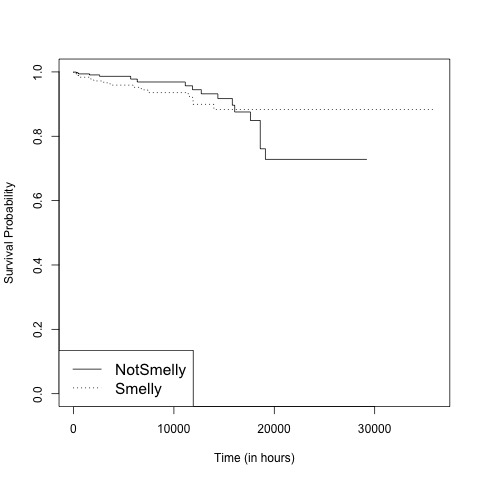
\epsfig{file = pdfs/Express_vulnerabilities_smells_file-grain_rplot.jpg, width = 4cm}}%
	}
	\subfigure[request.js]{%
		{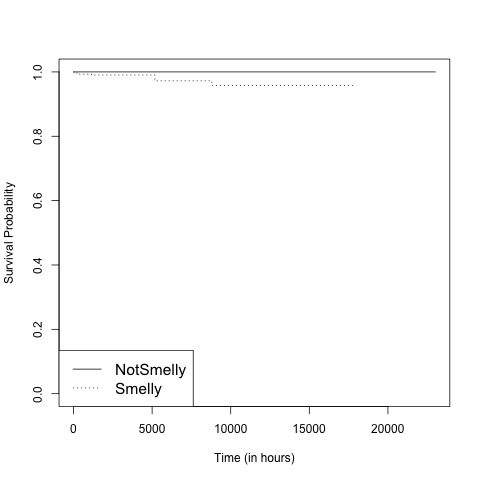
\epsfig{file = pdfs/Request_vulnerabilities_smells_file-grain_rplot.jpg, width = 4cm}}%
	}
	\subfigure[grunt.js]{%
		{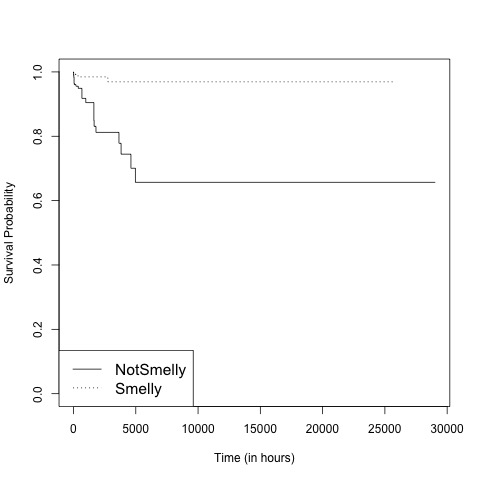
\epsfig{file = pdfs/Grunt_vulnerabilities_smells_file-grain_rplot.jpg, width = 4cm}}%
	}
	\subfigure[bower.js]{%
		{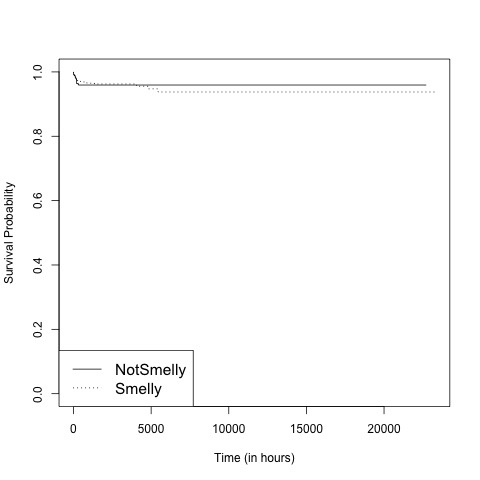
\epsfig{file = pdfs/Bower_vulnerabilities_smells_file-grain_rplot.jpg, width = 4cm}}%
	}
	\subfigure[hexo.js]{%
		{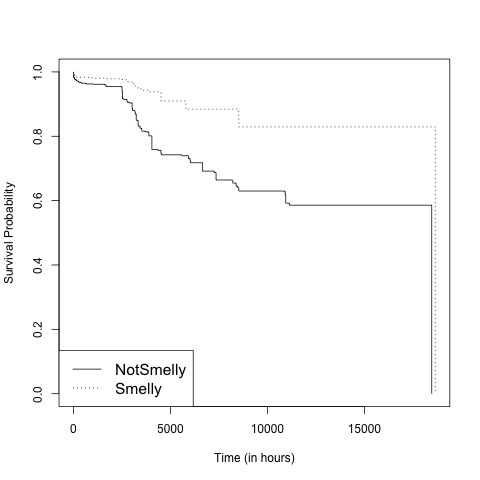
\epsfig{file = pdfs/Hexo_vulnerabilities_smells_file-grain_rplot.jpg, width = 4cm}}%
	}
	\subfigure[riot.js]{%
		{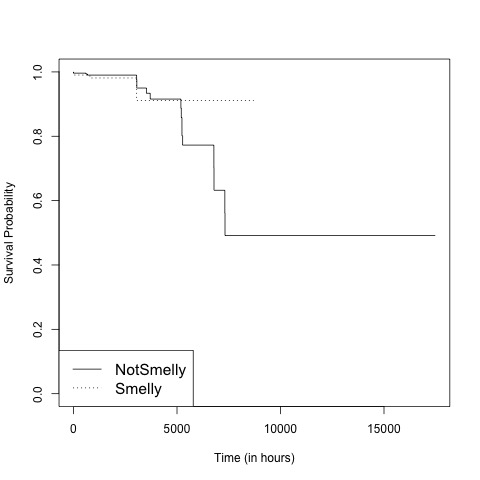
\epsfig{file = pdfs/Riot_vulnerabilities_smells_file-grain_rplot.jpg, width = 4cm}}%
	}
	\subfigure[webpack.js]{%
		{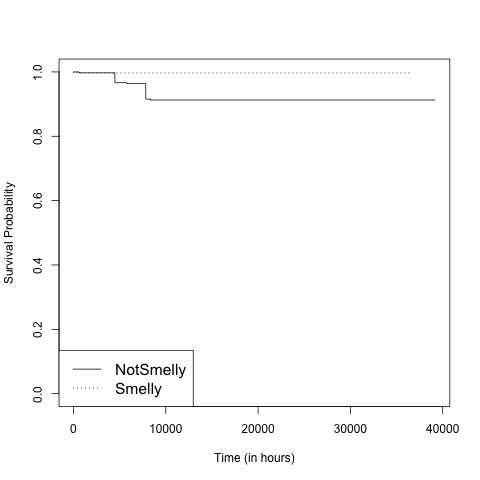
\epsfig{file = pdfs/Webpack_vulnerabilities_smells_file-grain_rplot.jpg, width = 4cm}}%
	}
	\subfigure[webtorrent.js]{%
		{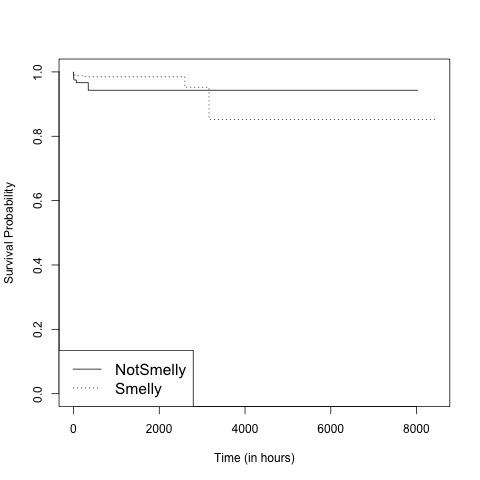
\epsfig{file = pdfs/Webtorrent_vulnerabilities_smells_file-grain_rplot.jpg, width = 4cm}}%
	}
	\caption{Survival probability trends of smelly codes vs. non-smelly codes in our fifteen JavaScript projects with the file grain approach (vulnerability study).\vspace{-10pt}}
	\label{rq3}
\end{figure*}

\begin{table*}[t]
	\centering
	\scriptsize
	\caption{Hazard ratios (vulnerability study) for each project with the line grain approach. $exp(coef)$ values means higher hazard rates.}
	\label{vulnlinegrain}
	\begin{tabular}{l|l|l|l}
		\hline
		module & $exp(coef)$ & $p$-value (Cox hazard model) & $p$-value (Proportional hazards assumption)     \\ \hline
		express  & 0.288 & 0.082e-3 & 0.113 \\ \hline
		request  & 0.189 & 0.014 & 0.441 \\ \hline
		bower	 & 0.229 & 0.031e-7 & 0.021 \\ \hline
		grunt    & 0.043 & 0.023e-7 & 0.994 \\ \hline
		hexo	 & 0.287 & 0.056e-14 & 0.902 \\ \hline
		webpack	 & 0.142 & 0.047e-3 & 0.089 \\ \hline
		webtorrent & 0.175 & 0.097e-3 & 0.217 \\ \hline
		riot	 & 0.774 & 0.445 & 0.505 \\ \hline
	\end{tabular}

\end{table*}

\begin{table*}[t]
	\centering
	\scriptsize
	\caption{Hazard ratios (vulnerability study) for each project with the line grain including dependencies approach. $exp(coef)$ values means higher hazard rates.}
	\label{vulnlinegraindep}
	\begin{tabular}{l|l|l|l}
		\hline
		module & $exp(coef)$ & $p$-value (Cox hazard model) & $p$-value (Proportional hazards assumption)     \\ \hline
		express  & 0.489 & 0.013 & 0.066 \\ \hline
		request  & 0.831 & 0.818 & 0.667 \\ \hline
		bower	 & 0.243 & 0.013e-6 & 0.009 \\ \hline
		grunt    & 0.096 & 0.03e-7 & 0.58 \\ \hline
		hexo	 & 0.322 & 0.04e-12 & 0.896 \\ \hline
		webpack	 & 0.176 & 0.09e-3 & 0.059 \\ \hline
		webtorrent & 0.31 & 0.009 & 0.109 \\ \hline
		riot	 & 0.774 & 0.445 & 0.505 \\ \hline
	\end{tabular}

\end{table*}

\textbf{Approach}. We use here our framework described in Section~\ref{extraction} {\color{blue}(Figure~\ref{process2})} to collect information about the occurrence of the 12 studied code smells in our {\color{blue}fifteen} subject systems, as well as the vulnerable codes and commits.
For each file and for each revision $r$ (\ie{} corresponding to a commit), we also compute the \textbf{Time} and \textbf{Smelly} metrics defined in \textbf{RQ1}. We also compute the \textbf{Event}, but differently to \textbf{RQ1}: for the file grain approach, this metric takes the value $1$ if the revision $r$ introduces a vulnerability $v$ for the first time through its changes and $0$ otherwise. Indeed, We only take in account the revision $r$ in which the vulnerability $v$ appears for the first time. We use the SZZ algorithm to insure that the file contained a code smell when the vulnerability was introduced for the first time. For the line grain and line grain including dependencies approaches, this metric takes the value $1$ if the revision $r$ introduces the vulnerability $v$ for the first time and if there is at least one match between the vulnerable lines and the smell lines, and $0$ otherwise. Actually, if there is no matching, we say that there is no link between the changes that inroduce the vulnerability for the first time and the code smells.

To collect information about vulnerabilities of revisions, we question a specific vulnerability database, Snyk\footnote{https://snyk.io/test}, which gives us the vulnerabilities's characteristics of each revision and of each studied systems. However, this database is not complete, which poses two problems to keep in mind during our study:
\begin{itemize}
	\item Given a studied system, some of its revisions are not identified in the database. We often meet a situation in which three successive revisions should introduce a same vulnerability, but the intermediate one indexes no vulnerability because it is not recognized by the database.
	\item Some of our studied systems (more precisely seven, which means almost half) have no vulnerability. However, we are aware that this kind of system (which means large system) are unlikely to have no vulnerability. Thereby, we will focus our analyzes on the following eight systems: \textsl{bower}, \textsl{express}, \textsl{grunt}, \textsl{hexo}, \textsl{request}, \textsl{riot}, \textsl{webpack}, and \textsl{webtorrent}.
\end{itemize}
Also, this database presents another drawback, because of its low accuracy. Indeed, when a vulnerability is found by the database, it does not specify any file of the revision in which the vulnerability has been found. Thus, we can only suppose that the vulnerability affects all the files changed by the revision, which is not accurate.

Using the smelly metric, in a similar way than \textbf{RQ1}, we divide our dataset in two groups: one group containing files with code smells (\ie{} smelly = 1) and another group containing files without any of the 12 studied code smells (\ie{} smelly = 0). For each group we create an individual Cox hazard model. In each group, the covariate of interest (\ie{} smelly) is a constant function (with value either 1 or 0), hence, there is no need for a link function to establish a linear relationship between this covariate and our event of interest, \ie{} the first appearance of a vulnerability. We use the \textsl{survfit} and \textsl{coxph} functions from R~\cite{rPackage} to analyze our Cox hazard models.

In addition to building Cox hazard models, we test the following null hypothesis: \emph{$H^{2}_{0}$: There is no difference between the probability of a first vulnerability occurrence in a file containing code smells and a file without code smells}. We use the \textsl{log-rank} test (which compares the survival distributions of two samples), to accept or refute this null hypothesis.

\textbf{Findings}. File grain results presented in Figure~\ref{rq3} show that files containing code smells don't necessarily experience vulnerability faster than files without code smells (only \textsl{request} and \textsl{bower} show that files containing smells have a trend to be more vulnerable than files without smells). Table~\ref{vulnlinegrain} (line grain results) and~\ref{vulnlinegraindep} (line grain including dependencies results) show the same accentuated observation, because none of the \textsl{exp(coef)} is greater than $1$. The $Y$-axis in Figure~\ref{rq3} represents the probability of a file \emph{surviving} a vulnerability occurrence. Hence a low value on the $Y$-axis means a low \emph{survival} rate (\ie{} a high vulnerability or high risk of vulnerability occurrence).  
For all fifteen projects, and for each approach (file grain, line grain, and line grain including dependencies), we calculated relative fault hazard rates (using Equation~\ref{eq3} from Section~\ref{survival}) between files containing code smells and files without code smells. Results show that, on average, files without code smells have hazard rates 34\% upper than files with code smells in our file grain analysis, and this pourcentage increases with the others analyzes (line grain and line grain including dependencies). Nevertheless, we need to be careful with our conclusion because of the lack of completeness and accuracy of our vulnerability database, as said previously. Hence, we can not reject $H^{2}_{0}$ because of our \textsl{exp(coef)} results, but we can not validate it because of the weaknesses of the vulnerability database we used.

\hypobox{JavaScript files with code smells are not necessarily more vulnerable than JavaScript files without code smells, and we need a better vulnerability database to confirm or refute more precisely our conclusion.}

\subsection*{(RQ4) Are JavaScript files with code smells equally vulnerable?}

\begin{table}[t]
	\centering
	\scriptsize
	\caption{Hazard ratios (vulnerability study) for each type of code smells with file grain approach. Higher $exp(coef)$ values means higher hazard rates.}
	\begin{tabular}{c|c|c|p{1.1cm}|p{1.3cm}}
		\hline
		module & covariate & $exp(coef)$ & $p$-value (Cox hazard model) & $p$-value (Proportional hazards assumption) \\ \hline
		\multirow{1}{*}{grunt} 
		& Variable Re-assign & 0.178 & 0.057e-5 & 0.169 \\ \hline
		\multirow{2}{*}{request}
		& LOC & 1.002 & 0.001 & 0.935 \\ \cline{2-5}
		& This Assign & 4.707 & 0.03 & 0.52 \\ \hline
		\multirow{2}{*}{hexo}
		& This Assign & 0.41 & 0.02 & 0.275 \\ \cline{2-5}
		& Variable Re-assign & 0.407 & 0.074e-8 & 0.668 \\ \hline
		\multirow{1}{*}{riot}
		& This Assign & 2.76 & 0.026 & 0.974 \\ \hline
		\multirow{1}{*}{webpack}
		& LOC & 1.001 & 0.009 & 0.465 \\ \hline
	\end{tabular}
	\label{smelltypes4}

\end{table}

\begin{table}[t]
	\centering
	\scriptsize
	\caption{Hazard ratios (vulnerability study) for each type of code smells with line grain approach. Higher $exp(coef)$ values means higher hazard rates.}
	\begin{tabular}{c|c|c|p{1.1cm}|p{1.3cm}}
		\hline
		module & covariate & $exp(coef)$ & $p$-value (Cox hazard model) & $p$-value (Proportional hazards assumption) \\ \hline
		\multirow{1}{*}{express}
		& Variable Re-assign & 0.342 & 0.001 & 0.08  \\ \hline
		\multirow{1}{*}{grunt} 
		& Variable Re-assign & 0.047 & 0.059e-7 & 0.996 \\ \hline
		\multirow{1}{*}{bower}
		& This Assign & 0.283 & 0.015 & 0.756 \\ \hline
		\multirow{2}{*}{request}
		& LOC & 1.002 & 0.001 & 0.935 \\ \cline{2-5}
		& Variable Re-assign & 0.228 & 0.028 & 0.426 \\ \hline
		\multirow{3}{*}{hexo}
		& This Assign & 0.291 & 0.006 & 0.377 \\ \cline{2-5}
		& Chained Methods & 0.2 & 0.023 & 0.593 \\ \cline{2-5}
		& Variable Re-assign & 0.297 & 0.014e-12 & 0.868 \\ \hline
		\multirow{2}{*}{webpack}
		& LOC & 1.001 & 0.009 & 0.465 \\ \cline{2-5}
		& Variable Re-assign & 0.146 & 0.061e-3 & 0.088 \\ \hline
		\multirow{1}{*}{webtorrent}
		& Variable Re-assign & 0.24 & 0.002 & 0.183 \\ \hline
	\end{tabular}
	\label{smelltypes5}

\end{table}

\begin{table}[t]
	\centering
	\scriptsize
	\caption{Hazard ratios (vulnerability study) for each type of code smells with line grain including dependencies approach. Higher $exp(coef)$ values means higher hazard rates.}
	\begin{tabular}{c|c|c|p{1.1cm}|p{1.3cm}}
		\hline
		module & covariate & $exp(coef)$ & $p$-value (Cox hazard model) & $p$-value (Proportional hazards assumption) \\ \hline
		\multirow{1}{*}{grunt} 
		& Variable Re-assign & 0.088 & 0.057e-7 & 0.581 \\ \hline
		\multirow{1}{*}{bower}
		& This Assign & 0.283 & 0.015 & 0.756 \\ \hline
		\multirow{1}{*}{request}
		& LOC & 1.002 & 0.001 & 0.935 \\ \hline
		\multirow{2}{*}{hexo}
		& This Assign & 0.291 & 0.006 & 0.377 \\ \cline{2-5}
		& Variable Re-assign & 0.327 & 0.035e-11 & 0.972 \\ \hline
		\multirow{2}{*}{webpack}
		& LOC & 1.001 & 0.009 & 0.465 \\ \cline{2-5}
		& Variable Re-assign & 0.181 & 0.012e-2 & 0.058 \\ \hline
	\end{tabular}
	\label{smelltypes6}

\end{table}

\textbf{Approach}. Similar to \textbf{RQ3}, we use our framework from Section~\ref{extraction} (Figure~\ref{process2}) to collect information about the occurrence of the 12 studied code smells, as well as the vulnerable codes and commits, in our fifteen studied systems. For each file and for each revision $r$ (\ie{} corresponding to a commit), we also compute the \textbf{Time} and \textbf{Event} metrics defined in \textbf{RQ3}. For each type of code smell $i$ we define the metric \textbf{Smelly$_{i}$:} which takes the value $1$ if the revision $r$ of the file contains the code smell $i$ and $0$ if it doesn't contain any of the 12 studied code smells. Also, for the line grain and the line grain including dependencies approaches, we define the metric \textbf{Event$_{i}$:} which takes the value $1$ if the revision $r$ introduces a vulnerability $v$ for the first time through its changes and if the code smell $i$ is in the intersection between the vulnerability lines and the smell lines, and $0$ otherwise. When computing the \textbf{Event} and \textbf{Event$_{i}$} metrics, we used the SZZ algorithm to ensure that the file contained the code smell $i$ when the vulnerability was introduced.
Because size and code churn could be related to vulnerability, we add the following metrics to our models, to control for the effect of these covariates : (i) LOC: the number of lines of code in the file at revision $r$; (ii) Code Churn: the sum of added, removed and modified lines in the file prior to revision $r$.

We perform a stratification considering the covariates mentioned above, in order to monitor their effect on our event of interest, \ie{} a vulnerability occurrence. Next, we create a Cox hazard model for each of our fifteen studied systems.
We then generated summaries of all our Cox hazard models and removed insignificant covariates, \ie{} those with $p$-values greater than $0.05$. Finally, for each system, we performed a non-proportional test to verify if the proportional hazards assumption holds. 

\textbf{Findings}. Tables~\ref{smelltypes4},~\ref{smelltypes5} and~\ref{smelltypes6} summarize the vulnerability hazard ratios for the 12 studied code smells for respectively the file grain, line grain, and line grain including dependencies approach. The value in the column \textsl{exp(coef)} shows the amount of increase in vulnerability hazard rate that one should expect for each unit increase in the value of the corresponding covariate.
The last column of Tables~\ref{smelltypes4},~\ref{smelltypes5} and~\ref{smelltypes6} show that the $p$-values obtained for the non-proportionality tests are above $0.05$ for all the fifteen systems; meaning that the proportional hazards assumption is satisfied for all the fifteen studied systems. Actually, we removed from the tables the insignificant covariates, which means those with non-proportionality test $p$-values less than $0.05$.

Overall, the vulnerability hazard ratios of the studied code smells vary across the systems and accross the approaches (file grain, line grain and line grain including dependencies), and almost all of them have an \textsl{exp(coef)} less than $1$. It confirms our last conclusion in \textbf{RQ3}, that is to say that JavaScript files with code smells are not more vulnerable than those without code smells (and we still have to mitigate this conclusion because of our vulnerability database). As said in \textbf{RQ3}, we collected information only on eight systems (out of fifteen) because of the lack of completeness of the vulnerability database. Plus, because of our $p$-values restriction, only a few covariates are reported in our tables, and some of the eight studied systems don't appear. However, it is interesting to notice that with the file grain approach, \textsl{This Assign} has the highest vulnerability hazard ratio in three out of eight systems (37.5\%), and is the only covariate with a hazard ratio greater than $1$ in two systems (\textsl{request} and \textsl{riot}); \textsl{Variable Re-assign} has one of the highest hazard rate in two out of eight systems (25\%); \textsl{This Assign} and \textsl{Variable Re-assign} are the only smell covariates reported. With our line grain approach, \textsl{Variable Re-assign} has still one of the highest hazard ratio in most systems, that is to say in six out of eight systems (75\%); \textsl{This Assign} has one of the highest hazard rate in two out of eight systems (25\%); \textsl{Chained Methods} is the most hazard code smell in only one out of eight systems (12.5\%); the other smells don't appear in any of the studied systems because of the $p$-values limitations. With the line grain including dependencies approach, \textsl{Variable Re-assign} is still one of the most hazard code smell in most systems, in three out of fifteen systems (37.5\%); \textsl{This Assign}  has one of the highest hazard rate in two out of eight systems (25\%); and only \textsl{Variable Re-assign} and \textsl{This Assign} are reported. Furthemore, the most vulnerability hazard types of code smell seem not to vary accross the approaches, and this observation particularly affects \textsl{Variable Re-assign} and \textsl{This Assign} code smells.

In our three approaches, the covariate LOC is significantly related to fault occurrence in two systems (\textsl{request} and \textsl{webpack}) with a very low hazard rate, meaning that JavaScript developers cannot simply control for size if they want to track vulnerable files effectively. Since \textsl{Variable Re-assign} and \textsl{This Assign} have the highest hazard ratios in respectively 46\% and 29\% of the cases (which means eight studied systems and three approches, that is to say $24$ cases), we can recommend that developers prioritize files containing these two types of code smells in order to make their system less vulnerable. \textsl{Variable Re-assign} seems, as in \textbf{RQ2}, an unavoidable type smell that developers have to strongly consider when they maintain, test, and fix their system for reducing fault-proneness and potentially vulnerability.

\hypobox{JavaScript files containing different types of code smells are not equally vulnerable. Developers should consider refactoring files containing \textsl{Variable Re-assign} code smell or \textsl{This Assign} code smell in priority since they seem to increase the risk of vulnerability in the system. Finally, \textsl{Variable Re-assign} code smell is essential to consider for reducing the risk of vulnerability and fault in the system.}

\subsection*{(RQ5) How do the smells survive over time?}

\begin{table*}[!htbp]
	\centering

	\caption{Descriptive statistics on survival over time of the largest smells of studied systems.}
	\begin{tabular}{c|c|c|c|c|c|c}
		\hline
		System & Smell & Not Survived & Survived & Number created at file birth & Median days or survival & Average days of survival \\ \hline
		\multirow{5}{*}{express}
		& Variable Re-assign & 6743 & 425 & 5783 (80.7\%) & 74 & 209 \\ \cline{2-7}
		& Nested Callbacks & 314 & 728 & 417 (40\%) & 1101 & 1152 \\ \cline{2-7}
		& Complex Code & 374 & 5 & 353 (93.1\%) & 74 & 122 \\ \cline{2-7}
		& Long Methods & 283 & 9 & 260 (89\%) & 74 & 143 \\ \cline{2-7}
		& SUM & 8430 & 1238 & 7348 (76\%) & & \\ \hline
		\multirow{5}{*}{grunt} 
		& Variable Re-assign & 2210 & 317 & 1636 (64.7\%) & 248 & 411 \\ \cline{2-7}
		& Lengthy Lines & 243 & 108 & 172 (49\%) & 248 & 681 \\ \cline{2-7}
		& Complex Code & 91 & 5 & 83 (85.4\%) & 248 & 292 \\ \cline{2-7}
		& Long Methods & 55 & 5 & 41 (68.3\%) & 248 & 334 \\ \cline{2-7}
		& SUM & 2732 & 448 & 2017 (63.4\%) & & \\ \hline
		\multirow{5}{*}{bower}
		& Variable Re-assign & 1427 & 1801 & 1235 (38.3\%) & 797 & 777 \\ \cline{2-7}
		& Chained Methods & 82 & 96 & 35 (19.7\%) & 1231 & 819 \\ \cline{2-7}
		& Lengthy Lines & 32 & 50 & 28 (34.1\%) & 644 & 719 \\ \cline{2-7}
		& Nested Callbacks & 38 & 32 & 27 (38.6\%) & 163 & 656 \\ \cline{2-7}
		& SUM & 1647 & 2087 & 1368 (36.6\%) & & \\ \hline
		\multirow{5}{*}{less}
		& Variable Re-assign & 36979 & 3779 & 37303 (91.5\%) & 56 & 281 \\ \cline{2-7}
		& Assign. in Cond. State. & 1349 & 4 & 1261 (93.2\%) & 405 & 477 \\ \cline{2-7}
		& Lengthy Lines & 547 & 26 & 509 (88.8\%) & 36 & 139 \\ \cline{2-7}
		& This Assign & 392 & 33 & 387 (91.1\%) & 129 & 314 \\ \cline{2-7}
		& SUM & 40241 & 3927 & 40391 (91.4\%) & & \\ \hline
		\multirow{5}{*}{request}
		& Variable Re-assign & 1362 & 667 & 1140 (56.2\%) & 365 & 534 \\ \cline{2-7}
		& This Assign & 28 & 50 & 34 (43.6\%) & 874 & 743 \\ \cline{2-7}
		& Chained Methods & 32 & 22 & 38 (70.4\%) & 256 & 557 \\ \cline{2-7}
		& Nested Callbacks & 1 & 28 & 1 (3.4\%) & 774 & 592 \\ \cline{2-7}
		& SUM & 1455 & 777 & 1232 (55.2\%) & & \\ \hline
		\multirow{5}{*}{jquery}
		& Variable Re-assign & 13076 & 5156 & 12122 (66.5\%) & 528 & 694 \\ \cline{2-7}
		& Complex Switch Case & 146 & 15 & 130 (80.7\%) & 179 & 435 \\ \cline{2-7}
		& This Assign & 118 & 37 & 120 (77.4\%) & 539 & 716 \\ \cline{2-7}
		& Chained Methods & 59 & 58 & 35 (29.9\%) & 657 & 785 \\ \cline{2-7}
		& SUM & 13743 & 5356 & 12675 (66.4\%) & & \\ \hline
		\multirow{5}{*}{hexo}
		& Variable Re-assign & 19023 & 823 & 17626 (88.8\%) & 2 & 86 \\ \cline{2-7}
		& Lengthy Lines & 768 & 12 & 675 (86.5\%) & 10 & 138 \\ \cline{2-7}
		& Long Parameter List & 755 & 3 & 728 (96\%) & 2 & 20 \\ \cline{2-7}
		& Complex Code & 599 & 19 & 576 (93.2\%) & 2 & 51 \\ \cline{2-7}
		& SUM & 22522 & 980 & 20584 (87.6\%) & & \\ \hline
		\multirow{5}{*}{leaflet}
		& Variable Re-assign & 5856 & 498 & 2241 (35.3\%) & 789.5 & 734 \\ \cline{2-7}
		& Lengthy Lines & 733 & 270 & 358 (35.7\%) & 203 & 354 \\ \cline{2-7}
		& Nested Callbacks & 123 & 489 & 114 (18.6\%) & 986 & 1029 \\ \cline{2-7}
		& Long Methods & 77 & 5 & 32 (39\%) & 911 & 752 \\ \cline{2-7}
		& SUM & 6997 & 1278 & 2855 (34.5\%) & & \\ \hline
		\multirow{5}{*}{ramda}
		& Variable Re-assign & 4720 & 1078 & 4656 (80.3\%) & 375 & 391 \\ \cline{2-7}
		& Chained Methods & 365 & 101 & 344 (73.8\%) & 241 & 372 \\ \cline{2-7}
		& Long Parameter List & 176 & 90 & 208 (78.2\%) & 206 & 396 \\ \cline{2-7}
		& Complex Code & 194 & 28 & 200 (90.1\%) & 375 & 364 \\ \cline{2-7}
		& SUM & 5668 & 1340 & 5599 (79.9\%) & & \\ \hline
		\multirow{5}{*}{chart}
		& Variable Re-assign & 5297 & 5696 & 4538 (41.3\%) & 406 & 365 \\ \cline{2-7}
		& This Assign & 199 & 388 & 86 (14.7\%) & 406 & 339 \\ \cline{2-7}
		& Lengthy Lines & 119 & 14 & 34 (25.6\%) & 12 & 154 \\ \cline{2-7}
		& Complex Switch Case & 53 & 30 & 31 (37.3\%) & 169 & 258 \\ \cline{2-7}
		& SUM & 5740 & 6207 & 4746 (39.7\%) & & \\ \hline
		\multirow{5}{*}{riot}
		& Variable Re-assign & 8331 & 2625 & 7866 (71.9\%) & 52 & 188 \\ \cline{2-7}
		& Lengthy Lines & 193 & 33 & 206 (91.2\%) & 7 & 150 \\ \cline{2-7}
		& This Assign & 63 & 92 & 61 (39.4\%) & 43 & 110 \\ \cline{2-7}
		& Assign. in Cond. State. & 107 & 47 & 80 (51.9\%) & 100.5 & 196 \\ \cline{2-7}
		& SUM & 9119 & 2937 & 8637 (71.6\%) & & \\ \hline
		\multirow{5}{*}{vue}
		& Variable Re-assign & 4199 & 5833 & 6587 (65.7\%) & 139 & 175 \\ \cline{2-7}
		& Lengthy Lines & 2947 & 4208 & 3518 (49.2\%) & 125 & 143 \\ \cline{2-7}
		& Complex Code & 414 & 675 & 679 (62.4\%) & 139 & 171 \\ \cline{2-7}
		& Long Methods & 259 & 417 & 421 (62.3\%) & 139 & 171 \\ \cline{2-7}
		& SUM & 8612 & 11712 & 12129 (59.7\%) & & \\ \hline
		\multirow{5}{*}{moment}
		& Variable Re-assign & 5642 & 11063 & 6154 (36.8\%) & 450 & 486 \\ \cline{2-7}
		& Nested Callbacks & 19 & 335 & 12 (3.4\%) & 492 & 464 \\ \cline{2-7}
		& Complex Switch Case & 117 & 69 & 114 (61.3\%) & 299 & 634 \\ \cline{2-7}
		& Chained Methods & 113 & 42 & 74 (47.7\%) & 243 & 389 \\ \cline{2-7}
		& SUM & 6135 & 11590 & 6561 (37\%) & & \\ \hline
		\multirow{5}{*}{webpack}
		& Variable Re-assign & 4643 & 627 & 3192 (60.6\%) & 352 & 593 \\ \cline{2-7}
		& Nested Callbacks & 379 & 54 & 276 (63.7\%) & 104 & 359 \\ \cline{2-7}
		& Chained Methods & 371 & 16 & 174 (45\%) & 492 & 589 \\ \cline{2-7}
		& Lengthy Lines & 182 & 38 & 86 (39.1\%) & 236 & 518 \\ \cline{2-7}
		& SUM & 5970 & 813 & 3987 (58.8\%) & & \\ \hline
		\multirow{5}{*}{webtorrent}
		& Variable Re-assign & 709 & 424 & 471 (41.6\%) & 335 & 370 \\ \cline{2-7}
		& This Assign & 108 & 53 & 88 (54.7\%) & 335 & 427 \\ \cline{2-7}
		& Nested Callbacks & 28 & 55 & 23 (27.7\%) & 453 & 406 \\ \cline{2-7}
		& Chained Methods & 12 & 2 & 9 (64.3\%) & 19.5 & 122 \\ \cline{2-7}
		& SUM & 869 & 535 & 591 (42.1\%) & & \\ \hline
	\end{tabular}
	\label{survivalsmells}
\end{table*}

\begin{figure*}[!htbp]
	\centering%
	\subfigure[Variable Re-Assign]{%
		{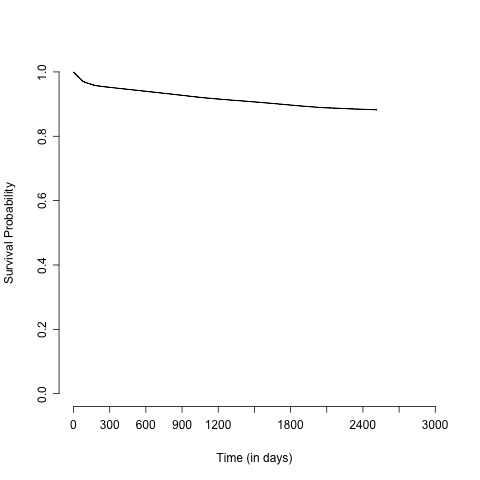
\epsfig{file = pdfs/Express_no-reassign_rplot.jpg, width = 4cm}}%
	}
	\subfigure[Nested Callbacks]{%
		{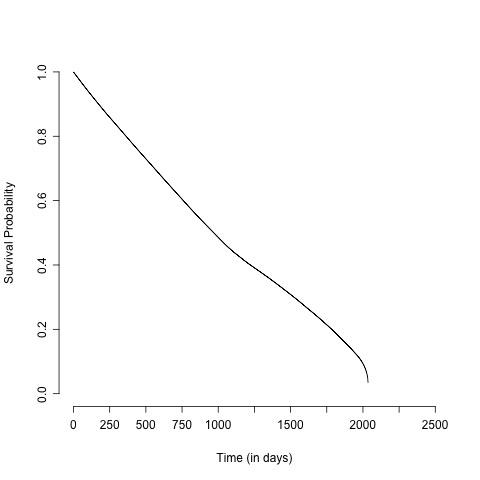
\epsfig{file = pdfs/Express_max-nested-callbacks_rplot.jpg, width = 4cm}}%
	}
	\subfigure[Complex Code]{%
		{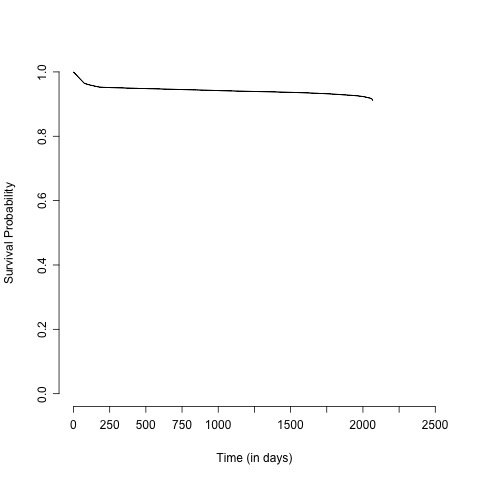
\epsfig{file = pdfs/Express_complexity_rplot.jpg, width = 4cm}}%
	}
	\subfigure[Long Methods]{%
		{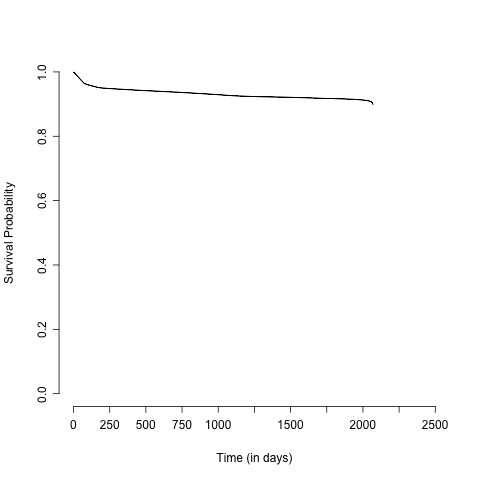
\epsfig{file = pdfs/Express_max-statements_rplot.jpg, width = 4cm}}%
	}
	\caption{Survival analyzes of the largest smells of express.js.\vspace{-10pt}}
	\label{survivalplots1}
\end{figure*}

\begin{figure*}[!htbp]
	\centering%
	\subfigure[Variable Re-Assign]{%
		{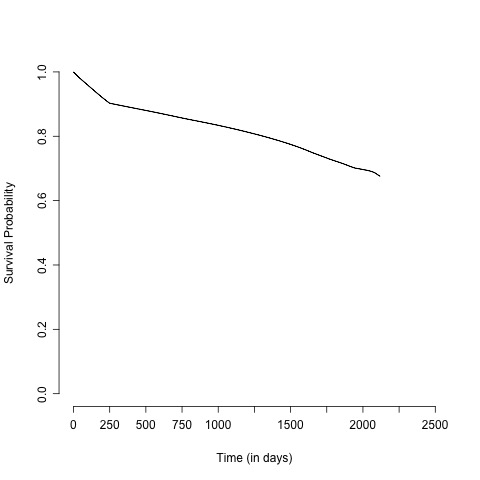
\epsfig{file = pdfs/Grunt_no-reassign_rplot.jpg, width = 4cm}}%
	}
	\subfigure[Lengthy Lines]{%
		{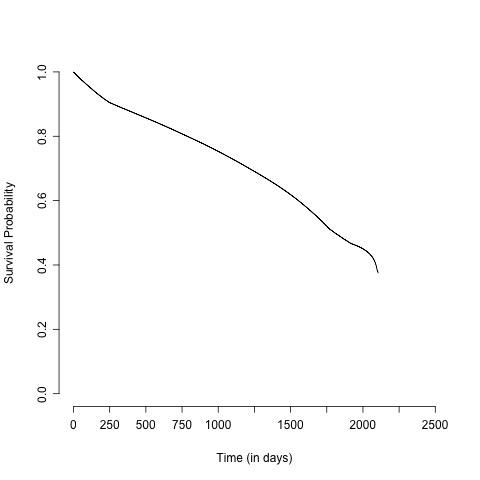
\epsfig{file = pdfs/Grunt_max-len_rplot.jpg, width = 4cm}}%
	}
	\subfigure[Complex Code]{%
		{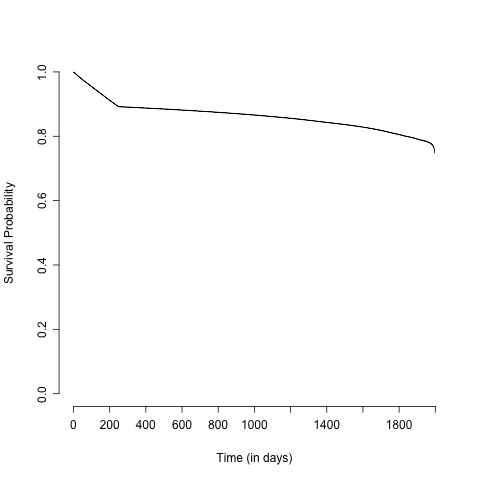
\epsfig{file = pdfs/Grunt_complexity_rplot.jpg, width = 4cm}}%
	}
	\subfigure[Long Methods]{%
		{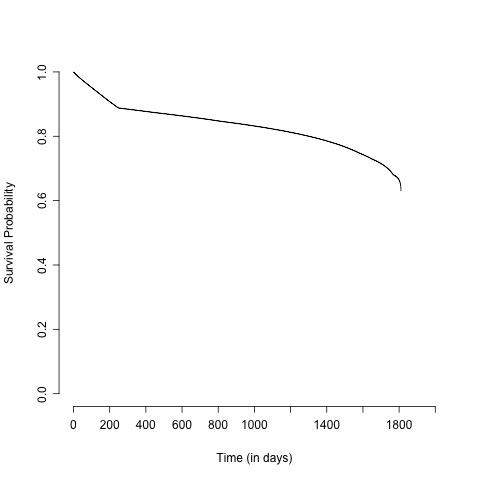
\epsfig{file = pdfs/Grunt_max-statements_rplot.jpg, width = 4cm}}%
	}
	\caption{Survival analyzes of the largest smells of grunt.js.\vspace{-10pt}}
	\label{survivalplots2}
\end{figure*}

\begin{figure*}[!htbp]
	\centering%
	\subfigure[Variable Re-Assign]{%
		{\epsfig{file = pdfs/Bower_no-reassign_rplot.jpg, width = 4cm}}%
	}
	\subfigure[Chained Methods]{%
		{\epsfig{file = pdfs/Bower_complex-chaining_rplot.jpg, width = 4cm}}%
	}
	\subfigure[Lengthy Lines]{%
		{\epsfig{file = pdfs/Bower_max-len_rplot.jpg, width = 4cm}}%
	}
	\subfigure[Nested Callbacks]{%
		{\epsfig{file = pdfs/Bower_max-nested-callbacks_rplot.jpg, width = 4cm}}%
	}
	\caption{Survival analyzes of the largest smells of bower.js.\vspace{-10pt}}
	\label{survivalplots3}
\end{figure*}

\begin{figure*}[!htbp]
	\centering%
	\subfigure[Variable Re-Assign]{%
		{\epsfig{file = pdfs/Less_no-reassign_rplot.jpg, width = 4cm}}%
	}
	\subfigure[Nested Callbacks]{%
		{\epsfig{file = pdfs/Less_max-nested-callbacks_rplot.jpg, width = 4cm}}%
	}
	\subfigure[Complex Code]{%
		{\epsfig{file = pdfs/Less_complexity_rplot.jpg, width = 4cm}}%
	}
	\subfigure[Long Methods]{%
		{\epsfig{file = pdfs/Less_max-statements_rplot.jpg, width = 4cm}}%
	}
	\caption{Survival analyzes of the largest smells of less.js.\vspace{-10pt}}
	\label{survivalplots4}
\end{figure*}

\begin{figure*}[!htbp]
	\centering%
	\subfigure[Variable Re-Assign]{%
		{\epsfig{file = pdfs/Request_no-reassign_rplot.jpg, width = 4cm}}%
	}
	\subfigure[This Assign]{%
		{\epsfig{file = pdfs/Request_this-assign_rplot.jpg, width = 4cm}}%
	}
	\subfigure[Chained Methods]{%
		{\epsfig{file = pdfs/Request_complex-chaining_rplot.jpg, width = 4cm}}%
	}
	\subfigure[Nested Callbacks]{%
		{\epsfig{file = pdfs/Request_max-nested-callbacks_rplot.jpg, width = 4cm}}%
	}
	\caption{Survival analyzes of the largest smells of request.js.\vspace{-10pt}}
	\label{survivalplots5}
\end{figure*}

\begin{figure*}[!htbp]
	\centering%
	\subfigure[Variable Re-Assign]{%
		{\epsfig{file = pdfs/Jquery_no-reassign_rplot.jpg, width = 4cm}}%
	}
	\subfigure[Complex Switch Case]{%
		{\epsfig{file = pdfs/Jquery_complex-switch-case_rplot.jpg, width = 4cm}}%
	}
	\subfigure[This Assign]{%
		{\epsfig{file = pdfs/Jquery_this-assign_rplot.jpg, width = 4cm}}%
	}
	\subfigure[Chained Methods]{%
		{\epsfig{file = pdfs/Jquery_complex-chaining_rplot.jpg, width = 4cm}}%
	}
	\caption{Survival analyzes of the largest smells of jquery.js.\vspace{-10pt}}
	\label{survivalplots6}
\end{figure*}

\begin{figure*}[!htbp]
	\centering%
	\subfigure[Variable Re-Assign]{%
		{\epsfig{file = pdfs/Hexo_no-reassign_rplot.jpg, width = 4cm}}%
	}
	\subfigure[Lengthy Lines]{%
		{\epsfig{file = pdfs/Hexo_max-len_rplot.jpg, width = 4cm}}%
	}
	\subfigure[Long Parameter List]{%
		{\epsfig{file = pdfs/Hexo_max-params_rplot.jpg, width = 4cm}}%
	}
	\subfigure[Complex Code]{%
		{\epsfig{file = pdfs/Hexo_complexity_rplot.jpg, width = 4cm}}%
	}
	\caption{Survival analyzes of the largest smells of hexo.js.\vspace{-10pt}}
	\label{survivalplots7}
\end{figure*}

\begin{figure*}[!htbp]
	\centering%
	\subfigure[Variable Re-Assign]{%
		{\epsfig{file = pdfs/Leaflet_no-reassign_rplot.jpg, width = 4cm}}%
	}
	\subfigure[Lengthy Lines]{%
		{\epsfig{file = pdfs/Leaflet_max-len_rplot.jpg, width = 4cm}}%
	}
	\subfigure[Nested Callbacks]{%
		{\epsfig{file = pdfs/Leaflet_max-nested-callbacks_rplot.jpg, width = 4cm}}%
	}
	\subfigure[Long Methods]{%
		{\epsfig{file = pdfs/Leaflet_max-statements_rplot.jpg, width = 4cm}}%
	}
	\caption{Survival analyzes of the largest smells of leaflet.js.\vspace{-10pt}}
	\label{survivalplots8}
\end{figure*}

\begin{figure*}[!htbp]
	\centering%
	\subfigure[Variable Re-Assign]{%
		{\epsfig{file = pdfs/Ramda_no-reassign_rplot.jpg, width = 4cm}}%
	}
	\subfigure[Chained Methods]{%
		{\epsfig{file = pdfs/Ramda_complex-chaining_rplot.jpg, width = 4cm}}%
	}
	\subfigure[Long Parameter List]{%
		{\epsfig{file = pdfs/Ramda_max-params_rplot.jpg, width = 4cm}}%
	}
	\subfigure[Complex Code]{%
		{\epsfig{file = pdfs/Ramda_complexity_rplot.jpg, width = 4cm}}%
	}
	\caption{Survival analyzes of the largest smells of ramda.js.\vspace{-10pt}}
	\label{survivalplots9}
\end{figure*}

\begin{figure*}[!htbp]
	\centering%
	\subfigure[Variable Re-Assign]{%
		{\epsfig{file = pdfs/Chart_no-reassign_rplot.jpg, width = 4cm}}%
	}
	\subfigure[This Assign]{%
		{\epsfig{file = pdfs/Chart_this-assign_rplot.jpg, width = 4cm}}%
	}
	\subfigure[Lengthy Lines]{%
		{\epsfig{file = pdfs/Chart_max-len_rplot.jpg, width = 4cm}}%
	}
	\subfigure[Complex Switch Case]{%
		{\epsfig{file = pdfs/Chart_complex-switch-case_rplot.jpg, width = 4cm}}%
	}
	\caption{Survival analyzes of the largest smells of chart.js.\vspace{-10pt}}
	\label{survivalplots10}
\end{figure*}

\begin{figure*}[!htbp]
	\centering%
	\subfigure[Variable Re-Assign]{%
		{\epsfig{file = pdfs/Riot_no-reassign_rplot.jpg, width = 4cm}}%
	}
	\subfigure[Lengthy Lines]{%
		{\epsfig{file = pdfs/Riot_max-len_rplot.jpg, width = 4cm}}%
	}
	\subfigure[This Assign]{%
		{\epsfig{file = pdfs/Riot_this-assign_rplot.jpg, width = 4cm}}%
	}
	\subfigure[Assignment in Conditional Statement]{%
		{\epsfig{file = pdfs/Riot_cond-assign_rplot.jpg, width = 4cm}}%
	}
	\caption{Survival analyzes of the largest smells of riot.js.\vspace{-10pt}}
	\label{survivalplots11}
\end{figure*}

\begin{figure*}[!htbp]
	\centering%
	\subfigure[Variable Re-Assign]{%
		{\epsfig{file = pdfs/Vue_no-reassign_rplot.jpg, width = 4cm}}%
	}
	\subfigure[Lengthy Lines]{%
		{\epsfig{file = pdfs/Vue_max-len_rplot.jpg, width = 4cm}}%
	}
	\subfigure[Complex Code]{%
		{\epsfig{file = pdfs/Vue_complexity_rplot.jpg, width = 4cm}}%
	}
	\subfigure[Long Methods]{%
		{\epsfig{file = pdfs/Vue_max-statements_rplot.jpg, width = 4cm}}%
	}
	\caption{Survival analyzes of the largest smells of vue.js.\vspace{-10pt}}
	\label{survivalplots12}
\end{figure*}

\begin{figure*}[!htbp]
	\centering%
	\subfigure[Variable Re-Assign]{%
		{\epsfig{file = pdfs/Moment_no-reassign_rplot.jpg, width = 4cm}}%
	}
	\subfigure[Nested Callbacks]{%
		{\epsfig{file = pdfs/Moment_max-nested-callbacks_rplot.jpg, width = 4cm}}%
	}
	\subfigure[Complex Switch Case]{%
		{\epsfig{file = pdfs/Moment_complex-switch-case_rplot.jpg, width = 4cm}}%
	}
	\subfigure[Chained Methods]{%
		{\epsfig{file = pdfs/Moment_complex-chaining_rplot.jpg, width = 4cm}}%
	}
	\caption{Survival analyzes of the largest smells of moment.js.\vspace{-10pt}}
	\label{survivalplots13}
\end{figure*}

\begin{figure*}[!htbp]
	\centering%
	\subfigure[Variable Re-Assign]{%
		{\epsfig{file = pdfs/Webpack_no-reassign_rplot.jpg, width = 4cm}}%
	}
	\subfigure[Nested Callbacks]{%
		{\epsfig{file = pdfs/Webpack_max-nested-callbacks_rplot.jpg, width = 4cm}}%
	}
	\subfigure[Chained Methods]{%
		{\epsfig{file = pdfs/Webpack_complex-chaining_rplot.jpg, width = 4cm}}%
	}
	\subfigure[Lengthy Lines]{%
		{\epsfig{file = pdfs/Webpack_max-len_rplot.jpg, width = 4cm}}%
	}
	\caption{Survival analyzes of the largest smells of webpack.js.\vspace{-10pt}}
	\label{survivalplots14}
\end{figure*}

\begin{figure*}[!htbp]
	\centering%
	\subfigure[Variable Re-Assign]{%
		{\epsfig{file = pdfs/Webtorrent_no-reassign_rplot.jpg, width = 4cm}}%
	}
	\subfigure[This Assign]{%
		{\epsfig{file = pdfs/Webtorrent_this-assign_rplot.jpg, width = 4cm}}%
	}
	\subfigure[Nested Callbacks]{%
		{\epsfig{file = pdfs/Webtorrent_max-nested-callbacks_rplot.jpg, width = 4cm}}%
	}
	\subfigure[Chained Methods]{%
		{\epsfig{file = pdfs/Webtorrent_complex-chaining_rplot.jpg, width = 4cm}}%
	}
	\caption{Survival analyzes of the largest smells of webtorrent.js.\vspace{-10pt}}
	\label{survivalplots15}
\end{figure*}

\textbf{Approach}. We use now the framework described in Section~\ref{extraction}, Figure~\ref{process3}, to collect information about the appearance of the 12 studied code smells in our fifteen subject systems, as well as their line localization, their content and their genealogy (which means their evolution over time from their creation to either their destruction, or the last revision of the studied system).
For each studied system and for each smell type, we compute the following metrics:
\begin{itemize}
	\item The number of created smells.
	\item The number of killed smells (over the system lifetime).
	\item The number of survived smells, which means the number of smell that presently appear in the system.
	\item The number of smells created at the file birthdate.
	\item The median days of survival of the smells.
	\item The average days of survival of the smells.
\end{itemize}
For each smell created (which means never encountered before), we also compute the \textbf{Time} and \textbf{Event} metrics thus defined: 
\begin{itemize}
	\item \textbf{Time:} the time in days since the smell creation.
	\item \textbf{Event:} this metric takes the value $1$ if the studied smell is present at this time (which means not killed), and $0$ otherwise.
\end{itemize}
In this way, if a particular smell $s$ is killed $x$ days after its introduction, we will have the corresponding event metric equal to $1$ from $0$ to $x-1$, and equal to $0$ at the time $x$ and after. When we report those information for a studied system, the maximum time that we take in account, for a particular smell type, corresponds to the maximum lifetime of the smells of this type. Thereby, for each smell type of the system and for each time, we will know the proportion of smells alive relatively to the number of smells created. This will particularly help us in the Cox survival model design.

Then, for each of the twelve studied smells, and for each of the fifteen studied systems, we create an individual Cox survival model using the \textbf{Time} and \textbf{Event} metrics previously defined. We use the \textsl{survfit} and \textsl{coxph} functions from R~\cite{rPackage} to analyze our Cox survival models.

\textbf{Findings}. Our results are presented in the Table~\ref{survivalsmells} for a density analysis, and in the Figures~\ref{survivalplots1} to~\ref{survivalplots15} for a survival analysis. 
For the Table~\ref{survivalsmells}, for each system and each smell, the third column corresponds to the number of killed smells, and the fourth to the number of survived smells. The sum of both columns gives us the number of created smells. The fifth column reports, in pourcentage, the proportion of smells created at the files birthdate, relatively to the number of created smells. In order to not overload the presentation of our results, we only report the descriptive statistics for the four most relevant smells, which means those for wich the number created is the most considerable. Finally, the Table reports, for each studied system, general statistics (\textsl{SUM} lines), computed by summing the statistics of the twelve studied smells.
For the Figures~\ref{survivalplots1} to~\ref{survivalplots15}, we plot the survival analysis for each studied systems, and for each smells reported in the Table~\ref{survivalsmells}, still in order to not overload the presentation of our results. The $Y$-axis corresponds to the chance of surviving of a given smell type, $x$ days after its introduction into the codebase.
The results presented in Table~\ref{survivalsmells} show that smells are not often introduced during files evolution and changes, but rather at the creation of files. Indeed, when we look at the \textsl{SUM} lines, from 34.5\% (for \textsl{leaflet}) to 91.4\% (for \textsl{less}) of the smells are introduced at the file birthdate, meaning that developers should be aware to their code when they create a JavaScript file, because it is precisely at this moment that most of the smells are introduced into the system. We also notice that, for the major part of the studied systems (eight out of fifteen), more than 20\% of the smells created still survive presently; and for thirteen systems, over than 10\% of the smells created are now present in those systems. It reveals that a significant part of the smells are never removed from the system once they are introduced in the code. Plus, after analyzing the commits of the studied systems, it is interesting to notice that most of time, the killed smells are removing at the same time than the file containing them (and not because of a file fix). The Table gives us also an overview of the smells lifetime, and we observe that for most of the systems (nine out of fifteen), the median and average days of survival of the most significant smell types are greater than $100$ days; and for fourteen systems out of fifteen (except \textsl{hexo}), at least one of the most sizable smell types has an average and median lifetime greater than $100$ days. This observation highlights that in general, smells tend to survive a very long time inside the system once they are introduced. Finally, Table~\ref{survivalsmells} presents an interesting result, which is that the smell \textsl{Variable Re-assign} is always the most considerable smell type (in our fifteen studied systems) in term of number of created smells, and its survival rate follows the trend of the sum of the smells (when we consider all the created smells of the system). For every studied system, over $1000$ \textsl{Variable Re-assign} smells are created, and for eight systems out of fifteen, the number of created smells of this type exceeds $10000$. Once again, \textsl{Variable Re-assign} is at the heart of our analysis, because as said previously, it is one of the most risky smell in terms of fault-proneness and vulnerability.
According to our Figures~\ref{survivalplots1} to~\ref{survivalplots15}, the four most significant smell types of each studied system have a considerable chance of surviving $500$ days after their introduction. This is indeed the case for all the most significant smell types for nine systems out of fifteen (except \textsl{request}, \textsl{chart}, \textsl{moment}, \textsl{webtorrent}, and \textsl{vue}), with over $50$\% chance of surviving $500$ days after the introduction of their largest smell types. Also, for fourteen studied systems out of fifteen (except \textsl{vue}), at least one of the most sizable smell types has more than $50$\% chance of surviving $500$ days after its smells introduction. Plus, for twelve systems out of fifteen (except \textsl{bower}, \textsl{vue}, and \textsl{webtorrent}), the \textsl{Variable Re-assign} smell type has over than $50$\% chance of surviving $1500$ days after its introduction. These observations show the trend of the smells of the studied systems to be persistent and survive a long time after their were introduced into the code, and also the significance of \textsl{Variable Re-assign} which is strongly linked to fault-proneness, and is the most proliferated smell type in the studied systems with a very high chance of surviving over time.

\hypobox{Most of the studied smells (from 34.5\% to 91.4\%) are introduced during the creation of JavaScript files. Once introduced, in most of half of the cases (eight systems), over than 20\% of the studied smells are not removed and have a high chance of surviving a very long time. Plus, \textsl{Variable Re-assign}, which is the most subject to fault-proneness and vulnerability, is also the most sizable smell type with the highest chance of surviving over time.}

}
\section{Perceived Criticality of Code Smells by JavaScript Developers}\label{survey}
To understand the perception of developers towards our studied code smells, we conducted a qualitative study with JavaScript developers. In total 1,484 developers took part in our qualitative study. The survey consisted of 3 questions about the participant background and 15 questions about the studied code smells. We designed a website \footnote{https://srvy.online/js} to run the survey. The study took place between October 4\ts{th} and October 17\ts{th}, 2016. The link to the survey was shared within the \emph{Hacker News community} \footnote{https://news.ycombinator.com/} and the \emph{EchoJS community} \footnote{http://www.echojs.com/}. Participants were free to skip any question and they could leave the survey at any time. However, none of the participants used the skip button. 68\% of the participants to our survey had more than 3 years of experience writing Javascript applications. We asked the participants about their usages of JavaScript and found that 92\% of them use JavaScript to write client-side applications and 51\% use it for server side applications. Over 63\% of participants were familiar with the concept of \emph{code smell} and 19\% never heard of it.

The results of our survey showed that 20\% of participants use pure callbacks to handle asynchronous logic, while 66\% use \emph{Promises} and 13\% use the newest ES6 and ES7 features to control the flow of asynchronous codes. 92\% of participants indicated that nesting the callbacks makes the code harder to maintain.

86\% of our participants reported that they prefer codes using \texttt{const} instead of \texttt{var} to declare variables and not re-using them in the same scope. 73\% indicated that re-using variables makes the code harder to maintain.

Surprisingly, 74\% of our participants said they preferred having assignments in conditional statements while using \emph{Regular Expressions}, however, 54\% of them acknowledged that this practice makes the code harder to maintain.

55\% of our participants reported that they prefer using \texttt{.bind(this)} instead of assigning \texttt{this} to other variables. However, only 16\% of the participants indicated that they use \texttt{.bind}. 55\% of the participants indicated that they use \emph{arrow functions} to have lexical \texttt{this}.

Although the JavaScript documentation lists \emph{Complex Switch Case} as a code smell, only 14\% of our participants preferred \texttt{if/else} structures over \texttt{switch/case}.

In the survey, we asked participants to rank the 12 studied code smells on a Likert scale from 1 to 10, based on their impact on the software understandability, debugging and maintenance efforts. Results show that participants consider \emph{Nested Callbacks} to be the most hazardous code smells (with a rating of 8.1/10), followed by \emph{Variable Re-assign} (with a rating of 6.5/10) and \emph{Long Parameter List} (with a rating of 6.2/10). They claimed that these code smells negatively affect the maintainability and reliability of JavaScript systems. This assessment is in line with the findings of our quantitative analysis.

%\Foutse{please add more information about the survey here, the background of the developers, the period on which the survey was conducted ... a link to the online questionnaire and summarize the results of the survey explain how they agree or disagree with the results of your quantitative analysis...}

%Developers that took part in our survey ranked ``nested callbacks", ``variable-reassing" and ``max-param" as the most harmful code smells. They claimed that these code smells negatively affect the maintainability and reliability of JavaScript systems. An assessment in line with the findings of our quantitative analysis. % This result confirms our quantitative analysis in which the code smells increase the defect-proneness and different smells have different effects weights.

%The \emph{variable-reassing} code smell appeared in both of our quantitative and qualitative study as one of the top hazardous smells.


\section{Threats to validity}\label{threats}

In this section, we discuss the threats to validity of our study following common guidelines for empirical studies~\cite{robert2002case}.

\textbf{Construct validity threats} concern the relation between theory and observation. In our study, threats to the construct validity are mainly due to measurement errors. %Our metrics in our survival analysis might not reflect all characteristics related to defects \Foutse{do you mean code smells or faults?} and we could include more metrics specifically related to source code or even the review process of fault fixes. \Foutse{you should explain why your results are still valid regardless of this limitation!} %We leave the selection of more metrics as a future work.
The number of previous faults in each source code file was calculated by identifying the files that were committed in a fault fixing revision. This technique is not without flaws. We identified fault fixing commits by mining the logs searching for certain keywords (\ie{} ``bug",``fix"',``defect" and ``patch") as explained in Section~\ref{extraction}. Following this approach, we are not able to detect fault fixing revisions if the committer either misspelled the keywords or failed to include any commit message. Nevertheless, this heuristic was successfully used in multiple previous studies in software engineering~\cite{jaafar2013mining,shihab2013studying}. The SZZ heuristic used to identify fault-inducing commits is not 100\% accurate. However, it has been successfully used in multiple previous studies from the literature, with satisfying results. In our implementation, we remove all fault-inducing commit candidates that only changed blank or comment lines. When analyzing the \emph{smelliness} of files that experienced fault-inducing changes, we only tracked the presence of the smell in the file as a whole. Hence, the smell contained in the file may not have been involved in the changed lines that induced the fault. %we assume the a smell didn't get touched if it is removed from a section of a file and another added to another section of the same file in the same commit.}

\textbf{Internal validity threats} concern our selection of systems and tools. % other possible explanations for some of our observations. We used SZZ algorithm to find original commits that induced bugs later in the project. The SZZ algorithm is a an heuristic approach and might not contain all 100\% true positive original commits.
The metric extraction tool used in this paper is based on the AST provided by ESLint. The results of the study are therefore dependent on the accuracy of ESLint. However, we are rather assured that this tool functions properly as it is being used widely by big companies. \eg{} Facebook, Paypal, Airbnb.
%The threshold selected to find smelly codes is by top 10\%  ... The different numbers for threshold might change the category of files as smelly or not smelly. Hence, different strategies to define a threshold may lead different results at the end.
We chose a logarithmic link function for some of our covariates in the survival analysis. It is possible that a different link function would be a better choice for these covariates. However, the non-proportionality test implies that the models were a good fit for the data. %We leave the selection of different link functions for each covariate as future work.
Also, we do not claim causation in this work, we simply report observations and correlations and tries to explain these findings.

\textbf{Threats to conclusion validity} address the relationship between the treatment and the outcome. We are careful to acknowledge the assumptions of each statistical test.

\textbf{Threats to external validity} concern the possibility to generalize our results. In this paper, we have studied {\color{blue}fifteen} large JavaScript projects. We have also limited our study to open-source projects. Still, these projects represent different domains and various project sizes. Table~\ref{studiedsystems} shows a summary of the studied systems, their domain and their size. Nevertheless, further validation on a larger set of JavaScript systems, considering more types of code smells is desirable. %done to further validate our results. %\New{We have limited this study to a list of 12 types of code smells; however, the list includes the most common bad practices in JavaScript. Future works should also consider other types of code smells.}

\textbf{Threats to reliability validity} concern the possibly of replicating our study. In this paper, we provide all the details needed to replicate our study. All our {\color{blue}fifteen} subject systems are publicly available for study. The data and scripts used in this study is also publicly available on Github\footnote{https://github.com/DavidJohannesWall/smells\_project}.
%Therefore, we can not generalize 100\% our results to other JavaScript projects particularly closed-source ones. Even though our study includes a small subset of available JavaScript software, we attempted to mitigate this issues by selecting a diverse number of projects.

{\color{blue}
\textbf{Threats to internal genealogy construction} is about our way to get the smells genealogy of the studied smells, more specifically the recognition of the smells over time and commits. Indeed, we set a similarity threshold of 70\%, meaning that if two smells of the same type have a similarity greater than 70\%, there are likely the same. Obviously, this threshold is not perfect and can associate two different smells together, or dissociate two smells, which are in reality the same. However, we changed it in order to see if some significant differences would appear, but no relevant difference was revealed.
	
}

\section{Related Work}\label{sec:related}
In this section, we discuss the related literature on code smell and JavaScript systems.
Code Smells~\cite{fowler1997refactoring} are poor design and implementation choices that are reported to negatively impact the quality of software systems. They are opposite to design patterns~\cite{Gam95} which are good solutions to recurrent design problems.
%Other researches have been done on Javascript before. Most of the previous studies on Javascript have been done on client side security of Javascript applications. Saxena \ea developed a system to explore the execution space of client side Javascript applications to find security vulnerabilities \cite{saxena2010symbolic}. On the other study, they proposed a dynamic analysis technique to discover validation vulnerabilities in client side Javascript applications systematically \cite{saxena2010flax}. Richards \ea studied the dynamic behavior of Javascript by performing an empirical study on how and why the dynamic features of Javascript are being used \cite{richards2010analysis}. Bielova conducted a survey on Javascript security policies for client side applications and proposed a detailed comparision of the runtime monitoring based security technique for Javascript applications \cite{bielova2013survey}. Tripp and Weisman presented a hybrid-analysis solution to automate the assessment of Javascript client side application by combining white-box and black-box methodologies \cite{tripp2011hybrid}. Hallaraker \ea also proposed an approach based on monitoring Javascript code execution to detect malicious code behavior \cite{hallaraker2005detecting}.
The literature related to code smells generally falls into three categories: (1) the detection of code smells~(e.g.,~\cite{Khomh11-BGB,fard2013jsnose}); (2) the evolution of code smells in software systems (e.g.,~\cite{chatzigeorgiou2010investigating,CodeSmells_overtime,peters2012evaluating,tufano2015and}) and their impact on software quality (e.g., ~\cite{shatnawi2006investigation,khomh2012exploratory,Abbes11,jaafar2013mining,tufano2015and});
and (3) the relationship between code smells and software development activities (e.g.,~\cite{Sjoberg13QEC,Abbes11}).

Our work in this paper, {\color{blue}strongly related to the one of Amir Saboury et al.~\cite{saboury2017empirical}}, falls into the second category. We aim to understand how code smells affect the fault-proneness of JavaScript systems. Li and Shatnawi~\cite{shatnawi2006investigation} who investigated the relationships between code smells and the occurrence of errors in the code of three different versions of Eclipse reported that code smells are positively associated with higher error probability. In the same line of study, Khomh et al.~\cite{khomh2012exploratory} investigated the relationship between code smells and the change- and fault-proneness of 54 releases of four popular Java open source systems (ArgoUML, Eclipse, Mylyn and Rhino). They observed that classes with code smells tend to be more change- and fault-prone than other classes. Tufano et al. \cite{tufano2015and} investigated the evolution of code smells in 200 open source Java systems from Android, Apache, and Eclipse ecosystems and found that code smells are often introduced in the code at the beginning of the projects, by both newcomers and experienced developers. Sjoberg et al.~\cite{Sjoberg13QEC}, who investigated the relationship between code smells and maintenance effort reported that code smells have a limited impact on maintenance effort. However, Abbes et al.~\cite{Abbes11} found that code smells can have a negative impact on code understandability. Recently, Fard et al. \cite{fard2013jsnose} have proposed a technique named JNOSE to detect 13 different types of code smells in JavaScript systems. The proposed technique combines static and dynamic analysis. They applied JNOSE on 11 client-web applications and found ``lazy object" and ``long method/function" to be the most frequent code smells in the systems. WebScent~\cite{nguyen2012detection} is another tool that can detect client-side smells. It identifies mixing of HTML, CSS, and JavaScript, duplicate code in JavaScript, and HTML syntax errors. ESLint \cite{ESLint}, JSLint \cite{JslinT} and JSHint \cite{JSHint} are rule based static code analysis tools that can validate source codes against a set of best coding practices. Despite this interest in JavaScript code smells and the growing popularity of JavaScript systems, to the best of our knowledge, there is no study that examined the effect of code smells on the fault-proneness of JavaScript server-side projects. This paper aims to fill this gap. 

%These previous studies raised the awareness of the community about the potential negative impact of code smells on the quality of object oriented systems and recommended that developers apply refactorings to remove code smells from their systems. %of y recommend applying refactoring to remove such interactions of anti-patterns.

%Jaafar et al.~\cite{jaafar2013mining} examined the fault-proneness of classes sharing a static or a co-change relationship with a class containing a code smell and reported hat  an empirical study to analyze anti-patterns dependencies in more than 165000 commits of three Java open source software (ArgoUML, JFreeChart, and XerecesJ). They showed that, classes that have static relationship as well as the classes that have co-change relationship with anti-patterns are more likely to be fault-prone than others.

%and smelliness happens as a consequence of evolution and maintenance activities which can even be introduced by refactoring operations.  al.~\cite{Khomh:2012:ESI:2158916.2158921} show that there is a relation between antipatterns and the bug-proneness of a file. These studies provide empirical evidences on the relation between antipatterns and bugs.
%Khomh et al. \cite{khomh2012exploratory} who investigated the relationship between the presence of code smells and software change- and fault-proneness
%Tufano et al. \cite{tufano2015and} studied a large change history of 200 open source projects in Java (Android, Apache and Eclipse) and found that code smells can be formed since the beginning of a project by both newcomers and experienced deveopers and smelliness happens as a consequence of evolution and maintenance activities which can even be introduced by refactoring operations. Khomh et al. \cite{khomh2012exploratory} investigated the relationship between the presence of anti-patterns and software change- and fault-proneness on 54 releases of four popular Java open source systems (ArgoUML, Eclipse, Mylyn and Rhino). They discovered that classes with code smells tend to be more change-and fault-prone than the other classes. Jaafar et al. \cite{jaafar2013mining} conducted an empirical study to analyze anti-patterns dependencies in more than 165000 commits of three Java open source software (ArgoUML, JFreeChart, and XerecesJ). They showed that, classes that have static relationship as well as the classes that have co-change relationship with anti-patterns are more likely to be fault-prone than others.

%On the other hand, less studies aimed the quality and maintainability of Javascript applications \cite{nguyen2012detection}.
%A number of efforts have been done on tools that assist developers to better maintain their web applications. JSLint \cite{JslinT} is a static code analysis tool that can validate source codes against a set of best code practices. In a more closely related work, Fard et al. \cite{fard2013jsnose} proposed a technique that combines static with dynamic analysis to detect 13 different types of code smells. They applied their JNOSE on 11 web applications an found that ``lazy object" and ``long method/function" are amongst the most frequent code smells. WebScent ~\cite{nguyen2012detection} detects client-side smells and basically identifies mixing of HTML, CSS, and JavaScript, duplicate code in JavaScript, and HTML syntax error.
%
%However, non of mentioned works have examined the effect of code smells on a very important aspect of software, i.e., fault-proneness in JavaScript projects.

%Gizas \ea compared the latest release of 7 popular client side Javascript libraries and reported their overall quality, performance and validity \cite{gizas2012comparative}. Those studies however are only focused on the client side Javascript application.
%In this paper, we analyzed the quality of server side JavaScript applications and conduct an empirical study on five popular server side JavaScript frameworks over 537 releases to explore the survival of smelly codes in terms of catching software bugs.

%In the following sections we introduce the concept of NodeJS and NPM and discuss why this platform needs more attention in the researchers' community.

%\subsection*{JavaScript and Nodejs}
%\mytitle{JavaScript and Nodejs} JavaScript is a powerful, flexible and popular scripting programming language. It is the most commonly used programming language on both front-end and back-end with more than 90\% usage on the front-end and more than 54\% on the back-end \cite{so:survay2016}. It also has the most active repositories and total pushes on Github \cite{githut}.
%\Foutse{The systems investigated in this paper use NodeJS and NPM?} \Foutse{we need to explain why it is important to know these two concepts otherwise we should remove them...right now its not clear to me if they are useful for understanding the work presented in the paper, Amir please exlain.....}
%\mytitle{Nodejs} (also called Node) is an open source platform to run JavaScript on the server side. The core is based on Google's JavaScript runtime engine called V8. Node and V8 are mostly written in C and C++. Although V8 mainly supports running client-side JavaScript codes, Node uses its power to support long-running, real-time, scalable and memory efficient server-side network applications \cite{tilkov2010node}. Node is also famous for its event-driven nature and non-blocking I/O model, which makes it a perfect fit for data-intensive and network applications. On the first quarter of 2015, Joyent, IBM, Microsoft, PayPal, Fidelity, SAP and The Linux Foundation joined forces to bring neutral and open governance support to the Node community \cite{nodeFoundation}. The growing popularity of JavaScript raises the demand for good design practices and style-guides.

%\subsection*{NPM}
%\mytitle{NPM} Nodejs comes with its own package manager called NPM (Node Package Manager). NPM enables developers to install community libraries and their dependencies easily through the command-line interface \cite{tilkov2010node}. By the time of writing this paper, there are more than 310,000 distinct modules registered on NPM. With average growth rate of more than 400 modules per day, it is the most popular registry on the web \cite{modulecounts}. This shows how the popularity of using community libraries are increasing. NPm has increased the usage of community libraries drastically, thanks to its simple and easy to use APIs. % of NPM increased the usage of using community libraries drastically.
%Developers can add third-party modules as dependency of their application using simple commands. But, this raises the questions about the quality and security of those modules. In March 2016, a developer removed all of his modules from NPM. One of the modules called \texttt{left-pad}\footnote{https://www.npmjs.com/package/left-pad} had been used by thousands of other modules living in NPM. The removal of this small module with only 11 lines of code, broke thousands of other modules \cite{reg2016lp, med2016lp}. This event was a strong illustration of the impact that community modules can have on JavaScript applications. %is indicates how the security and quality of community modules impact JavaScript applications.




\section{Conclusion}\label{conclusion}

%In this paper, we developed an extension for ESLint in order to extract a set of code smells from five JavaScript projects. Then, we use Cox hazard models to find out whether smelly codes are harmful, and what specific types of code smells make it more defect-prone. We analyze the models to understand which covariates play significant roles in determining defects. We used log-rank test to measure whether a significant statistical difference exists between survival probabilities of smelly codes and non-smelly codes. We also demonstrate the validity and accuracy of our models using the non-proportionality assumption test. Moreover, we designed a survey to have JavaScript practitioners' opinions on the different types of source code practices, i.e., source codes with smells against source codes with the same rationale but without smells.
In this study, we examine the impact of code smells on the fault-proneness of JavaScript systems. {\color{blue}Also, we present a survival study of the smells of JavaScript systems.} We present a quantitative study of {\color{blue}fifteen} JavaScript systems that compare the time until a fault occurrence in JavaScript files that contain code smells and files without code smells, {\color{blue}with two different approaches: line grain, and line grain including dependencies approaches}. {\color{blue}This quantitative study also present some descriptive statistics about the twelve studied smells, as well as their survival by computing their lifetime.} Results show that JavaScript files without code smells have hazard rates {\color{blue}20\%} lower than JavaScript files with code smells {\color{blue}in the line grain study, and 38\% lower than JavaScript files with code smells in the line grain including dependencies study}. In other terms, the survival of JavaScript files against the occurrence of faults increases with time if the files do not contain code smells. We further investigated hazard rates associated with different types of code smells and found that ``Variable Re-assign", ``Assignment in Conditional Statements", {\color{blue}and ``Complex Code"} smells have the highest hazard rates. {\color{blue}The survival results show us that smells are introduced at the JavaScript files creation most of the time, and a big part of them still survived presently; those smells, and particularly ``Variable Re-assign" which is the most proliferated into the studied systems, have a high chance of surviving a very long time.} JavaScript developers should consider removing \emph{Variable Re-assign} code smells from their systems in priority since this code smell is consistently associated with a high risk of fault, {\color{blue}and because it is the most sizable code smell with a high chance of surviving over time}. They should also prioritize \emph{Assignment in Conditional Statements}, \emph{Complex Code}, \emph{This Assign}, \emph{Nested Callbacks}, and \emph{Long Parameter List} code smells for refactoring.

%
%  the occurenand a qualitative study by posting a survey among more than 1000 JavaScript developers, we have made two findings. First, we found that smelly code is more risky than non-smelly code; the risk seems to be system independent. We discovered that on average non-smelly codes have hazard rates 65\% lower than smelly codes. In other terms, the survival of all files against defects increases with time if they do not hold code smells. Second, in our findings we observed that all code smells do not equally affect software maintainability and reliability since variable-reassign (\textsl{var.reassign}) and assignment in condition (\textsl{cond.assign}) code smells have higher hazard rate in comparison to the other types of smells identified by our Cox model and survey.


%\textbf{Future work.}

%conference papers do not normally have an appendix

% use section* for acknowledgment
%\section*{Acknowledgment}
%The authors would like to thank... \cite{latexcompanion}

% trigger a \newpage just before the given reference
% number - used to balance the columns on the last page
% adjust value as needed - may need to be readjusted if
% the document is modified later
%\IEEEtriggeratref{8}
% The "triggered" command can be changed if desired:
%\IEEEtriggercmd{\enlargethispage{-5in}}

% references section

% can use a bibliography generated by BibTeX as a .bbl file
% BibTeX documentation can be easily obtained at:
% http://mirror.ctan.org/biblio/bibtex/contrib/doc/
% The IEEEtran BibTeX style support page is at:
% http://www.michaelshell.org/tex/ieeetran/bibtex/
%\bibliographystyle{IEEEtran}
% argument is your BibTeX string definitions and bibliography database(s)
%\bibliography{IEEEabrv,../bib/paper}
%
% <OR> manually copy in the resultant .bbl file
% set second argument of \begin to the number of references
% (used to reserve space for the reference number labels box)
%\begin{thebibliography}{1}

%\bibitem{IEEEhowto:kopka}
%H.~Kopka and P.~W. Daly, \emph{A Guide to \LaTeX}, 3rd~ed.\hskip 1em plus
%  0.5em minus 0.4em\relax Harlow, England: Addison-Wesley, 1999.

%\end{thebibliography}
\balance
\bibliographystyle{IEEEtran}
\bibliography{references}

% that's all folks
\end{document} 